%!TEX root = ../thesis.tex
%*******************************************************************************
%*********************************** Third Chapter *****************************
%*******************************************************************************
\cleardoublepage
\chapter{Kernel-based uncertainty quantification}
\label{chpt:3}
%*******************************************************************************
\hfill
\localtableofcontents
\newpage


\begin{tcolorbox}[colback=gray!5!white, colframe=gray!5!white, coltitle=gray!70!white, coltext=gray!60!white, title=\textbf{Parts of this chapter are adapted from the following references:}]
    A. Lovera, E. Fekhari, B. Jézéquel, M. Dupoiron, M. Guiton and E. Ardillon (2023). ``Quantifying and clustering the wake-induced perturbations within a wind farm for load analysis". In: \textit{Journal of Physics: Conference Series (WAKE 2023)}.\\

    E. Vanem, E. Fekhari, N. Dimitrov, M. Kelly, A. Cousin and M. Guiton (2023). ``A joint probability distribution model for multivariate wind and wave conditions''. In: \textit{Proceedings of the ASME 2023 42th International Conference on Ocean, Offshore and Arctic Engineering (OMAE 2023)}.
\end{tcolorbox}

%============================================================%
%============================================================%
\section{Introduction}
%============================================================%
%============================================================%
The main sources of solicitation in offshore design reside in the metocean conditions. 
To accurately verify a structural design against the joint wind and wave conditions, these random excitations must be carefully modelled. 
Offshore structures are usually certified against ultimate limit states (related to the occurrence of extreme metocean conditions) and fatigue limit states (related the average fatigue over the metocean conditions). 
In this context, the probabilistic framework is typically used to model the joint distribution of random variables describing the metocean conditions (listed in Section~\ref{sec:owt_uncertainties}). 

Note that a given probabilistic model might describe well the central behavior of the environmental distribution but not its tail behavior (and vice-versa).   
Extreme value theory develops specific methods to model the far tails of distributions \citep{beirlant_2006_extreme_values}. 
Modeling the tails is not the priority in the present work since the focus is on mean fatigue estimation.   

The environmental random variables studied present different particularities. 
First, an offshore wind turbine project leads to the collection of an important amount of metocean data (possibly merged with data from mesoscale simulations). 
Second, their dependence structure is complex, making the probabilistic modeling more complicated. 

This chapter explores different aspects of the environmental conditions' uncertainty quantification. 
The theory of some nonparametric copulas is introduced before their use in metocean conditions inference. 
A semiparametric approach is applied on the South Brittany data, mixing parametric modeling of the marginals with nonparametric modeling of the copula. 
To visually analyze multivariate distributions, the \textit{copulogram} is a new tool that decomposes the marginal effects and the dependence structure of a joint distribution. 

At the scale of a wind farm, each turbine perceives different metocean conditions as the wake of other turbines creates wind perturbations. 
To study this perturbation, an engineering wake model (see Section~\ref{sec:222}) was used to obtain one perturbed environmental distribution per turbine. 
This work applies a kernel-based discrepancy (the maximum mean discrepancy) to compare wake induced perturbations. 
In a second time, this discrepancy is used to gather wind turbines perceiving similar perturbations. 
This clustering can be used to perform uncertainty propagation at the farm scale by considering a few turbines with are representative of a cluster. 


%============================================================%
%============================================================%
\section{Dependence modeling with nonparametric copula}\label{sec:nonparametric_copula}
%============================================================%
%============================================================%

In uncertainty quantification, the lack of knowledge can lead to rough assumptions regarding the dependence modeling. 
However, an accurate representation of the uncertain inputs is of prime importance. 
For example, the work of \citet{torre_2019_copula_reliability} demonstrates the influence of the dependence model on the estimation of rare event probabilities by studying the same problem with different copula models. 

When inferring a probabilistic model over a multivariate dataset, one can decompose the problem into the fit of a set of marginals and the fit of a copula (see the Sklar Theorem \ref{thm:sklar}). 
In the case of metocean conditions, the fit of the marginals is not problematic considering the amounts of data available. 
However, the complex dependence structure appears to be more challenging. 
Different strategies to model the dependence for multivariate distributions are shortly summarized hereafter: 
\begin{itemize}
    \item \textbf{Vine copulas} (also known as pair copula) decompose the joint distribution as a product of conditioned bivariate copulas organized in a tree-like structure called a vine. 
    This approach proved to be very efficient, but it requires the definition of the vine and the bivariate parametric copulas \citep{joe2011dependence}. 
    \item \textbf{Conditional modeling} defines the joint distribution as a product of univariate conditional distributions. 
    In practice, the parameter of a marginal are defined as a function of other marginals (see e.g., \citealt{vanem_fekhari_2023}). 
    %This approach is widely used to model metocean conditions, but its implementation is not always straightforward. 
    \item \textbf{Multivariate KDE} is another way to capture the dependence together with marginal effects. As the dimension and the size of the dataset increase, this method become less tractable \citep{wand_jones_1994_kde}.  
    \item \textbf{Nonparametric copulas} are methods uniformly approximating an empirical copula without any assumption on a dependence structure. They will be further described and used for metocean conditions inference in the present chapter.    
\end{itemize}

\begin{remark}
    The strategy referred as ``conditional modeling'' can in fact be expressed as a copula \citep{vanem_2016} for continuous variables. For example, in the bivariate case of a continuous random vector $\bX = (X_1, X_2)$ with PDF $f_\bX(\bx)$, CDF $F_\bX(\bx)$ and density copula $c$: 
    \begin{subequations}
        \begin{align}
            f_\bX(\bx) &= f_{X_1}(x_1) \, f_{X_2|X_1}(x_2|x_1) = f_{X_1}(x_1) \, f_{X_2}(x_2) \, c\left(F_{X_1}(x_1), F_{X_2}(x_2)\right)\\
            \Leftrightarrow & c\left(F_{X_1}(x_1), F_{X_2}(x_2)\right) = \frac{f_{X_1}(x_1) \, f_{X_2|X_1}(x_2|x_1)}{f_{X_1}(x_1) \, f_{X_2}(x_2)}
        \end{align}  
    \end{subequations}
\end{remark}

The notions related to the copula theory are further introduced in the monographs of \citet{nelsen_2006_copulas,joe_2014,durante_2015_copula} while the key properties are introduced hereafter.


%============================================================%
\subsection{Preliminary definitions and properties}\label{sec:copula_prelims}
%============================================================%
%Soit X = (X 1 , . . . , X n ) T un vecteur aléatoire de dimension n défini sur l’espace
%n
%probabilisé (Ω, A, P) et soit x = (x 1 , . . . , x n ) T ∈ R une réalisation de X. La définition
%de copule est facilitée en introduisant les notions de face inférieure et bord supérieur
%de I n :
Let us consider a random vector $\bX \in \iD_{\bx}\subseteq\R^d$ defined on a probability space $(\Omega, \iA, \P)$. 
Its probability distribution $\P_\bX$ can be represented by a CDF $F_\bX$ and PDF $f_\bX$. 
The functional definition of a \textit{d-dimensional copula} (or simply ``d-copula'') is a density function $C:[0, 1]^d \mapsto [0, 1]$ whose marginals are uniformly distributed on $[0, 1]$.
\begin{theorem}[Copula]
    A function $C:[0, 1]^d \mapsto [0, 1]$ is a d-copula if, and only if, it presents the following properties:
    \begin{itemize}
        \item The function $C$ is ``grounded'' (also called ``anchored''): \\$C(u_1, \dots, u_d) = 0$ if $u_j=0, \, \forall j\in\{1, \dots, d\}$;
        \item The marginals of $C$ are uniform, then: $C(1, \dots, u_j, \dots, 1) = u_j,  \, \forall j\in\{1, \dots, d\}$;
        \item The function $C$ is ``d-increasing'', meaning that for any hyperrectangle $A \subset [0, 1]^d$, the corresponding volume induced by $C$ is positive (see \cite{durante_2015_copula} p.7). 
    \end{itemize}
    \label{thm:copula}
\end{theorem}

A copula is bounded by two functions according to the Fréchet-Hoeffding bounds. 
\begin{theorem}[Fréchet-Hoeffding bounds]
    If a function $C:[0, 1]^d \mapsto [0, 1]$ is a d-copula, then it respects the following bounds for all $\bu \in [0, 1]^d$: 
    \begin{equation}
        W(\bu) = \max (1 - d + u_1 + \dots + u_d, \, 0) \, \leq C(\bu) \, \leq \, M(\bu) = \min(u_1,\dots ,u_d).
    \end{equation} 
    Where the upper bound $M$ is still a copula while the lower bound $W$ is only one for $d=2$.
\end{theorem}

The rank transform plays an essential role to understand copulas. 
Considering a continuous random vector $\bX \in \iD_{\bx}$ and the sample $\bX_n = \left\{\bx^{(1)}, \dots, \bx^{(n)}\right\} \sim \bX$, its \textit{ranks} $\bR_n = \left\{\br^{(1)}, \dots, \br^{(n)}\right\} \in \N^{n}$ correspond to the indexes of its order statistics: 
\begin{equation}
    r^{(i)}_j = n \, \what{F}_{X_j}(x_j^{(i)}) = \sum_{l=1}^n \1_{\left\{x^{(l)}_j \leq x^{(i)}_j\right\}}, \quad \forall j \in \{1, \dots d\}, i \in \{1, \dots n\},
    \label{eq:ranks}  
\end{equation}
where $\what{F}_{X_j}$ stands for the marginal empirical CDF associated to the random variable $X_j$.


\begin{theorem}[Rank-invariance]
    Considering a random vector $\bX=(X_1, \dots, X_d)$, a set of mappings $\{r_j (\cdot)\}_{j=1}^d$, and the image random vector $\bR=(r_j \circ X_1, \dots, r_d \circ X_d)$. 
    If the mappings are strictly increasing (which is the case for the rank transform introduced in \eq{eq:ranks}), then, the copula associated to $\bR$ is invariant by transformation: $C_\bX = C_\bR$. 
    A proof is presented in \citet{durante_2015_copula} p. 57.
\end{theorem}

Transforming in the ranks generally reduces the effect of outliers and ensures more robust estimates. 
The invariance by rank transform of copulas allows the estimation of different \textit{dependence measures} in the ranked space. 


\paragraph{Spearman's rho.} Is a well-known dependence measure, also called the ``Spearman's rank correlation coefficient'', which is defined for two random variables $X_i, X_j$ as: 
\begin{equation}
    \rho^{\mathrm{S}}(X_i, X_j) = \frac{\cov(r_i(X_i), r_j(X_j))}{\sigma_{r_i(X_i)} \, \sigma_{r_j(X_j)}},
\end{equation}
an equivalent definition exists, using the copula $C$ between the joint distribution of $X_i$ and $X_j$ and the independent copula $\Pi(u_i, u_j) = u_i \, u_j$: 
\begin{equation}
    \rho^{\mathrm{S}}(X_i, X_j) = 12 \int_{[0, 1]^2} C(u_i, u_j) \, \dd u_i \dd u_j - 3 = 12 \int_{[0, 1]^2} (C(u_i, u_j) - \Pi(u_i, u_j)) \, \dd u_i \dd u_j. 
\end{equation}

\paragraph{Kendall's tau.} Also referred to as the ``Kendall's rank correlation coefficient'', is defined for a pair of random variables $(X_i, X_j)$ and their respective independent copies $(X_i', X_j')$ as: 
\begin{equation}
    \tau(X_i, X_j) = \P\left((X_i - X_i')(X_j - X_j') > 0 \right) - \P\left((X_i - X_i')(X_j - X_j') < 0 \right),
\end{equation}
and can also be defined using the copula $C$ between the joint distribution of the two random variables: 
\begin{equation}
    \tau(X_i, X_j) = 4 \int_{[0, 1]^2} C(u_i, u_j) \, \dd C(u_i, u_j) - 1 = 1 - 4 \int_{[0, 1]^2} \frac{\partial C(u_i, u_j)}{\partial u_i} \frac{\partial C(u_i, u_j)}{\partial u_j} \, \dd u_i \dd u_j 
\end{equation}
These dependence measures fully rely on the copula and are both bounded between -1 and 1. 
Further properties and estimators of Spearman's rho and Kendall's tau are presented in \citet{durante_2015_copula} Section 2.4. 


\paragraph{Upper/lower tail dependence.} Considering the random vector $\bX = (X_i, X_j)$ and the copula $C$ underlying their joint distribution. 
The \textit{upper/lower tail dependence} coefficients are defined as: 
\begin{subequations}
    \begin{align}
        \lambda_U(X_i, X_j) &= \lim_{\substack{u \rightarrow 1 \\ u<1}} \, \P\left(X_i > F_{X_i}^{-1}(u) | X_j > F_{X_j}^{-1}(u)\right) =       \lim_{\substack{u \rightarrow 1 \\ u<1}} \left(2 - \frac{1 - C(u, u)}{1 - u}\right)\\
        \lambda_L(X_i, X_j) &= \lim_{\substack{u \rightarrow 0 \\ u>0}} \, \P\left(X_i \leq F_{X_i}^{-1}(u) | X_j \leq F_{X_j}^{-1}(u)\right) = \lim_{\substack{u \rightarrow 0 \\ u>0}} \left(\frac{C(u, u)}{1 - u}\right) 
    \end{align}
\end{subequations}
\cite{joe_2014} further discusses asymptotic limit and outlines the particular case of the bivariate Gaussian copula, for which the tail dependence measures are null, $\lambda_U = \lambda_L = 0$.
Note that Kendall's tau and the tail dependence coefficients both have their associated plots, allowing to compare the dependence of two distributions \elias{add ref}.

%============================================================%
\subsection{Empirical and checkerboard copula}
%============================================================%

The \textit{empirical copula} was introduced by \citet{deheuvels_1979_empirical_copula}, as an estimator of the copula $C$ associated with the random vector $\bX$. 
Since the normalized ranks are a creasing mapping that present uniform marginals by construction, they are a natural empirical representation of the density copula. 
Considering a sample $\bX_n = \left\{\bx^{(1)}, \dots, \bx^{(n)}\right\} \sim \bX$ with the respective ranks $\bR_n = \left\{\br^{(1)}, \dots, \br^{(n)}\right\}$, a definition of the empirical copula is: 
\begin{equation}
    C_n(u_1, \dots, u_d) = \frac1n \sum_{i=1}^{n} \prod_{j=1}^{d} \1 \left\{ \frac{r_j^{(i)}}{n} \leq u_j \right\}, \quad  \bu = (u_1, \dots, u_d) \in [0, 1]^d
    \label{eq:empirical_copula}
\end{equation}
Even if this function converges uniformly towards the copula $C$ (according to the Glivenko-Cantelli theorem), it does not fulfill the conditions to be a copula (see e.g., \citealt{gonzalez_2021_checkerboard_copula}). 

In this context, different methods may be applied to smooth the empirical copula into a genuine copula. 
This problem can be perceived as a functional approximation of the underlying copula $C$, which is unique for continuous variables (according to Sklar's Theorem \ref{thm:sklar}). 
Let us consider a discretization of the unit hypercube as a grid: 
\begin{equation}
    G=\left\{\frac{0}{m_1}, \dots, \frac{m_1}{m_1}\right\} \times \dots \times \left\{\frac{0}{m_d}, \dots, \frac{m_d}{m_d}\right\}, \quad \bm = (m_1, \dots, m_d) \in \N^d. 
\end{equation}

The \textit{checkerboard copula} is a simple approximation of the empirical copula using the discretization $G$. 
This method is comparable to a multivariate histogram of the empirical density copula $c_n$ (see the formal multivariate definition proposed by \citealt{cottin_2014_bernstein}).
In the particular case for which $m_j=m, \, \forall j \in \{1, \dots, d\}$, the checkerboard copula is called the ``rook'' copula, and expressed by \citet{segers_2017} as: 
\begin{equation}
    C_n^{\#m}(u_1, \dots, u_d) = \frac1n \sum_{i=1}^{n} \prod_{j=1}^{d} \min\left(\max(n\, u_j - r_j^{(i)} +1, \, 0), \, 1\right).
\end{equation}

This empirical copula has a low complexity (see \citealt{rose_2015}) and efficient results for large samples \citep{gonzalez_2021_checkerboard_copula}, however, its variance is comparable to the empirical copula for small-sized samples \citep{segers_2017}. 
It is proven to be a genuine copula and its asymptotic behavior was studied by various authors such as \citet{li_1998_checkerboard,genest_2017_asymptotic_checkerboard}. 
In the following, an approximation of the empirical copula with Bernstein polynomials is presented. 



%============================================================%
\subsection{Empirical Bernstein and Beta copula}
%============================================================%

A few elements on Bernstein polynomials and their corresponding approximation is reminded before introducing the empirical Bernstein copula.

\subsubsection{Bernstein polynomials and approximation}
%------------------------------------------------------------%
Let us first define the \textit{Bernstein basis polynomial} of order $m \in \N$ as: 
\begin{equation}
    b_{m, t}(u)= \binom{m}{t}u^t(1-u)^{m-t}, \quad t \in \{0, \dots, m\}.
\end{equation}
These polynomials present various interesting properties, such as their nonnegativity over $[0, 1]$, being bounded by one, and offering a partition of unity on $[0, 1]$ \citep{lasserre_2023_bernstein}: 
\begin{equation}
    1 = \sum_{t=0}^{n} b_{m, t}(u)(x), \quad \forall x\in\R, \quad \forall n \in \N.
\end{equation} 

Bernstein's polynomials allow us to uniformly approximate any continuous and real-valued function defined on a compact set $f: [0, 1]^d \mapsto \R$ (as they were used to demonstrate the Weierstrass approximation theorem). 
In the multivariate case, the \textit{Bernstein approximation} of the function $f$ can be written on a grid over the unit hypercube $G=\left\{\frac{0}{m_1}, \dots, \frac{m_1}{m_1}\right\} \times \dots \times \left\{\frac{0}{m_d}, \dots, \frac{m_d}{m_d}\right\}, \bm = (m_1, \dots, m_d) \in \N^d$, as: 
\begin{equation}
    B_{\bm}(f)(\bu) = \sum_{t_1=0}^{m_1} \dots \sum_{t_d=0}^{m_d} f\left(\frac{t_1}{m_1}, \dots, \frac{t_d}{m_d}\right) \prod_{j=1}^d b_{m_j, t_j}(u_j) \, , \quad  \bu = (u_1, \dots, u_d) \in [0, 1]^d.
    \label{eq:bernstein_approx}
\end{equation}
The Bernstein polynomials approximate $f$ such that $\lim_{m\to\infty} B_{m}(f) = f$ uniformly on $\left[0,1\right]$. 


\subsubsection{Bernstein polynomials for copula approximation}
%------------------------------------------------------------%
Copulas are continuous and bounded functions defined on a compact set (the unit hypercube). 
Therefore, they are good candidates to be approximated by Bernstein polynomials. 
The Bernstein approximation applied on an empirical copula $C_n$ was introduced as \emph{empirical Bernstein copula} (EBC) by \cite{sancetta_satchell_2004} for applications in economics and risk management: 
\begin{equation}
    B_{\bm}(C_n)(\bu) = \sum_{t_1=0}^{m_1} \dots \sum_{t_d=0}^{m_d} C_n\left(\frac{t_1}{m_1}, \dots, \frac{t_d}{m_d}\right) \prod_{j=1}^d b_{m_j, t_j}(u_j) \, , \quad  \bu = (u_1, \dots, u_d) \in [0, 1]^d.
    \label{eq:ebc}
\end{equation}
In this expression, the evaluations of the empirical copula on the vertices of the grid are smoothed by the product of Bernstein polynomials. 
A respective approximation of the copula density can be directly expressed by deriving the previous formula. 
The EBC delivers a genuine copula, if and only if all the polynomial degrees $\{m_j\}_{j=1}^d$ are divisors of $n$ (see \citealt{segers_2017}, Proposition 2.5). 

In the particular case of regular grids, $\{m_j=m\}_{j=1}^d$, the EBC can be expressed as a mixture of beta distributions \citep{segers_2017}. 
Let us consider an $n$-sized rank sample, $\bR=(\br_1, \dots, \br_d) \in \N^{n}$, and the degree $m$ taken as divisor of $n$. 
Note that the r\textsuperscript{th} order statistic of an $n$-sized sample following a uniform $[0, 1]$ is distributed according to the beta distribution $\mathcal{B}(r, n-r+1)$. 
Considering these hypotheses, the EBC can be written as: 
\begin{equation}
    B_{m}(C_n)(\bu) = \frac 1n \sum_{i=1}^n \prod_{j=1}^{d} F_{m, r_j^{(i)}} \, , \quad  \bu = (u_1, \dots, u_d) \in [0, 1]^d, 
\end{equation}
where $F_{m, r}$ is the CDF of the beta distribution $\mathcal{B}(r, m-r+1)$ (also called the ``regularized incomplete beta function''): 
\begin{equation}
    F_{m, r} = \sum_{t=r}^{m} \binom{m}{t}u^t(1-u)^{m-t}, \quad u \in [0, 1], \quad r \in \{1, \dots, m\}. 
\end{equation}

Overall, the EBC is a very versatile tool which able to approximate complex dependence patterns. 
Moreover, Monte Carlo sampling on an EBC is straightforward and licit since it is a genuine copula. 
As a drawback, the estimation accuracy of this nonparametric method heavily relies on the polynomial order tuning.   


\subsubsection{Asymptotic behavior of the empirical Bernstein copula}
%------------------------------------------------------------%
In practice, the choice of polynomial degree for an EBC leads to a challenging bias-variance tradeoff. 
For example, the particular case of $\{m = n\}$, introduced as the \textit{empirical Beta copula} by \cite{segers_2017}, tends to reduce the bias while increasing the variance. 
In this paper, the beta copula presents interesting results compared to the Bernstein or the checkerboard copula for small sample sizes (i.e., $n<100$). 
Theoretically, the tuning of the degree was first optimized to minimize an ``Asymptotic Mean Integrated Squared Error'' (AMISE) of $B_{\bm}(C_n)$: 
\begin{equation}
    \mathrm{AMISE}(B_{\bm}(C_n)) = \E\!\left[ \lVert B_{\bm}(C_n) - C \rVert^2_2 \right] \!=\! \E\!\left[\!\int_{\R^d}\! \left(B_{\bm}(C_n)(\bu) \!-\! C(\bu) \dd \bu \right)^2 \!\right]\!\!.
    \label{eq:aimse}
\end{equation}
The seminal work of \citet{sancetta_satchell_2004} proves in Theorem 3 that: 
\begin{itemize}
    \item $B_{\bm}(C_n)(\bu) \rightarrow C(\bu)$ for any $u_j \in \left]0, 1\right[$ if $\frac{m^{d/2}}{n} \rightarrow 0$, when $m, n \rightarrow \infty$.
    \item The optimal polynomial order in terms of AMISE is\footnotemark: $m \lesssim m_{\mathrm{AIMSE}} = n^{2/(d+4)}, \forall u_j \in \left]0, 1\right[$.    
\end{itemize}
\footnotetext{The sign $\lesssim$ stands for ``less than or approximately''.}
To illustrate the previous theorem, \fig{fig:hmise} represents the evolution of the $m_{\mathrm{AMISE}}$ for different dimensions and sample sizes (adapted from \citealt{lasserre_2022}). 
In medium dimension, the values of $m_{\mathrm{IMSE}}$ tend towards one, which is equivalent to the independent copula. 
Therefore, high-dimensional problems should rather be divided into a product of smaller problems on which the EBC is tractable.

\begin{figure}
    \centering
    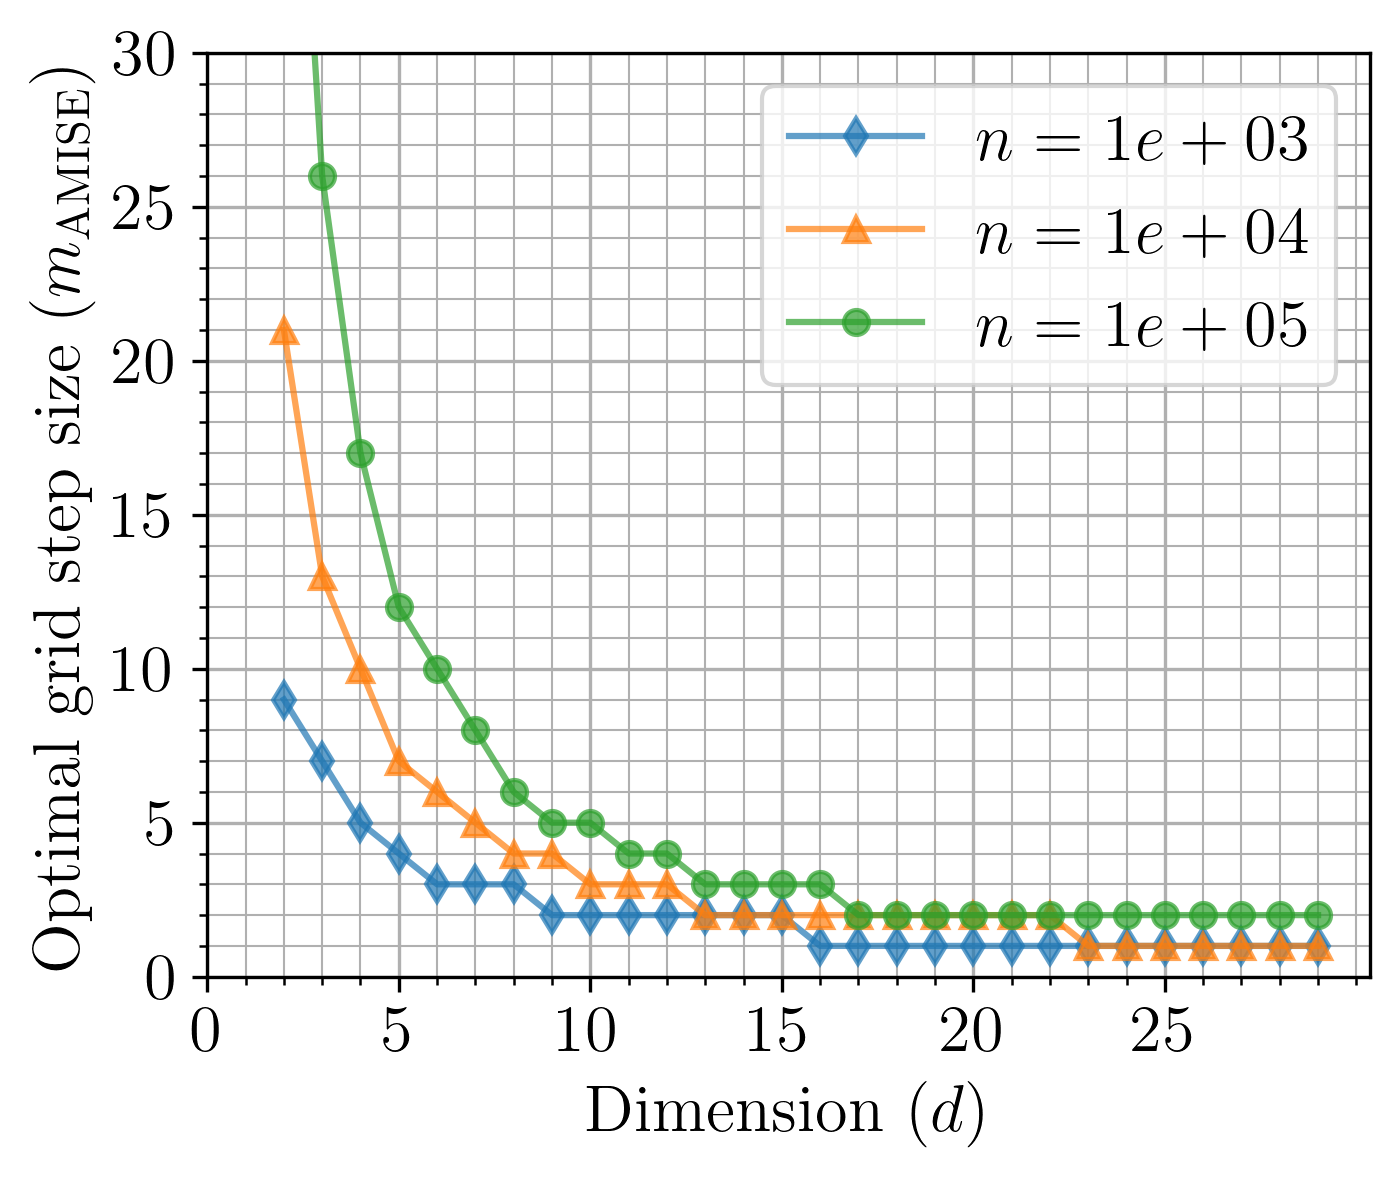
\includegraphics[width=0.5\linewidth]{../numerical_experiments/chapter3/figures/hAMISE.png}
    \caption{Evolution of $m_{\mathrm{IMSE}}$ for different dimensions and sample sizes.}
    \label{fig:hmise}
\end{figure}

The polynomial order for EBC estimation is still a bottleneck which was studied over the years by different authors (see e.g., \citealt{janssen_2012_ebc,bouezmarni_2013_EBC_convergence,rose_2015,segers_2017}).  
Meanwhile, other nonparametric approaches such as the ``penalized Bernstein'' and the ``penalized B-spline'' estimators were compared to the EBC and vine copulas in a benchmark realized by \citet{nagler_2017}. 
The results showed that the most performant methods vary depending on the problem studied (for different dimension, sample sizes, strength of dependence). 
Regarding tail dependence modeling, nonparametric approaches are generally limited, but recent contributions introduced Bootstrap procedures to better this aspect \citep{kiriliouk_2021_resampling}.


\subsubsection{Illustrative example on a Clayton copula}
%------------------------------------------------------------%
Let us consider a bivariate Clayton copula $C$ with parameter $\theta=2.5$ (see \citealt{nelsen_2006_copulas})
A Monte Carlo sample with size $n=10$ is generated on it, which is then used to build an empirical copula $C_n$ as defined in \eq{eq:empirical_copula}. 
\fig{fig:ebc_illustration} (a) illustrates the empirical copula corresponding to the sample, with the shade of grey matching the CDF values. 
Then, the Bernstein approximation of the empirical copula (i.e., the EBC)  is represented in \fig{fig:ebc_illustration} (b), (c), (d) according to the \eq{eq:ebc}. 
The three versions of the EBC correspond to different polynomial orders, assuming that $(m_1=m_2)$. 

As the order increases, the bias between the EBC and the copula $C$ tends to be reduced. 
Note that the second EBC in \fig{fig:ebc_illustration} (c) where $(m_1=m_2=n)$ is equivalent to the Beta copula. 
Moreover, increasing the order beyond the sample size definitely overfits of the copula. 

%\elias{possible alternative: 2D plots in two rows. Row 1: empirical copula/EBCn=5/EBCn=10. Row 2: empirical density copula/EBCn=5/EBCn=10.}

\begin{figure}
    \begin{subfigure}[b]{0.49\textwidth}
        \centering
        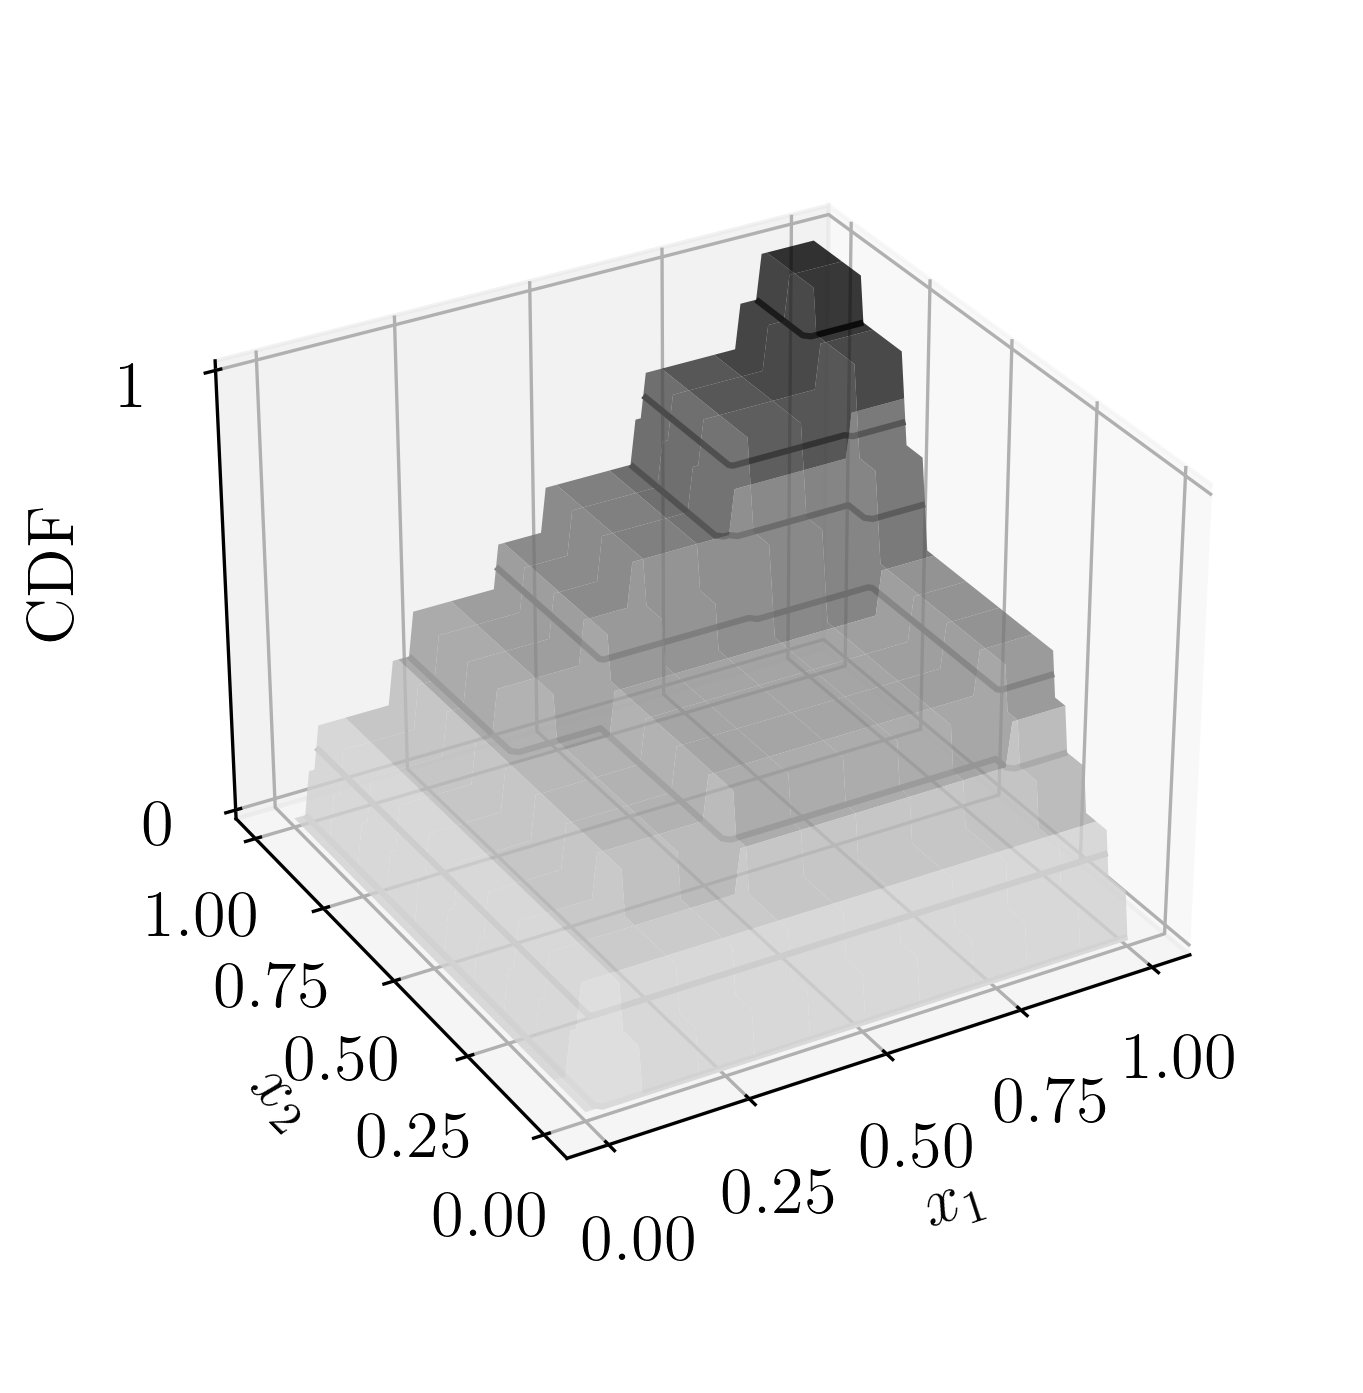
\includegraphics[width=\linewidth]{../numerical_experiments/chapter3/figures/empirical_copula.png}
        \caption{Empirical copula $C_n$ with ($n=10$).}
    \end{subfigure}
    \begin{subfigure}[b]{0.49\textwidth}
        \centering
        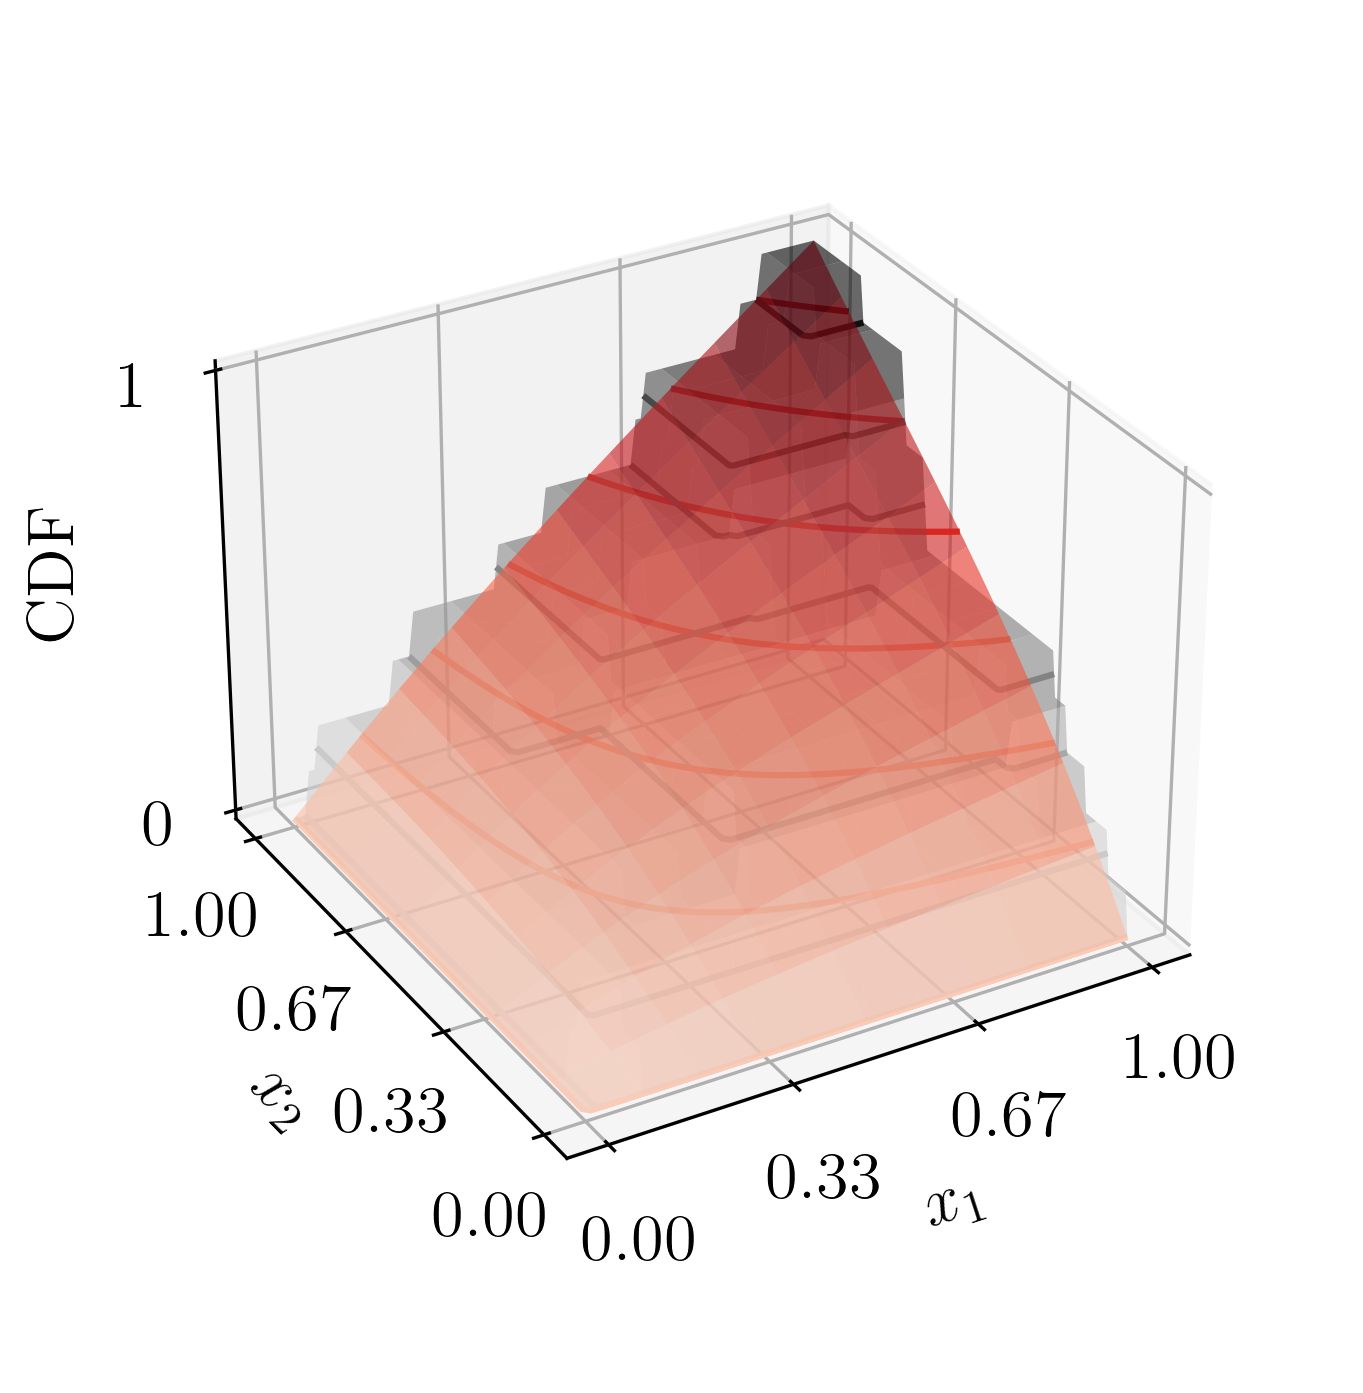
\includegraphics[width=\linewidth]{../numerical_experiments/chapter3/figures/ebc_m3.png}
        \caption{$B_{\bm}(C_n)$ with $(m_1=m_2=3)$.}
    \end{subfigure}
    \\
    \begin{subfigure}[b]{0.49\textwidth}
        \centering
        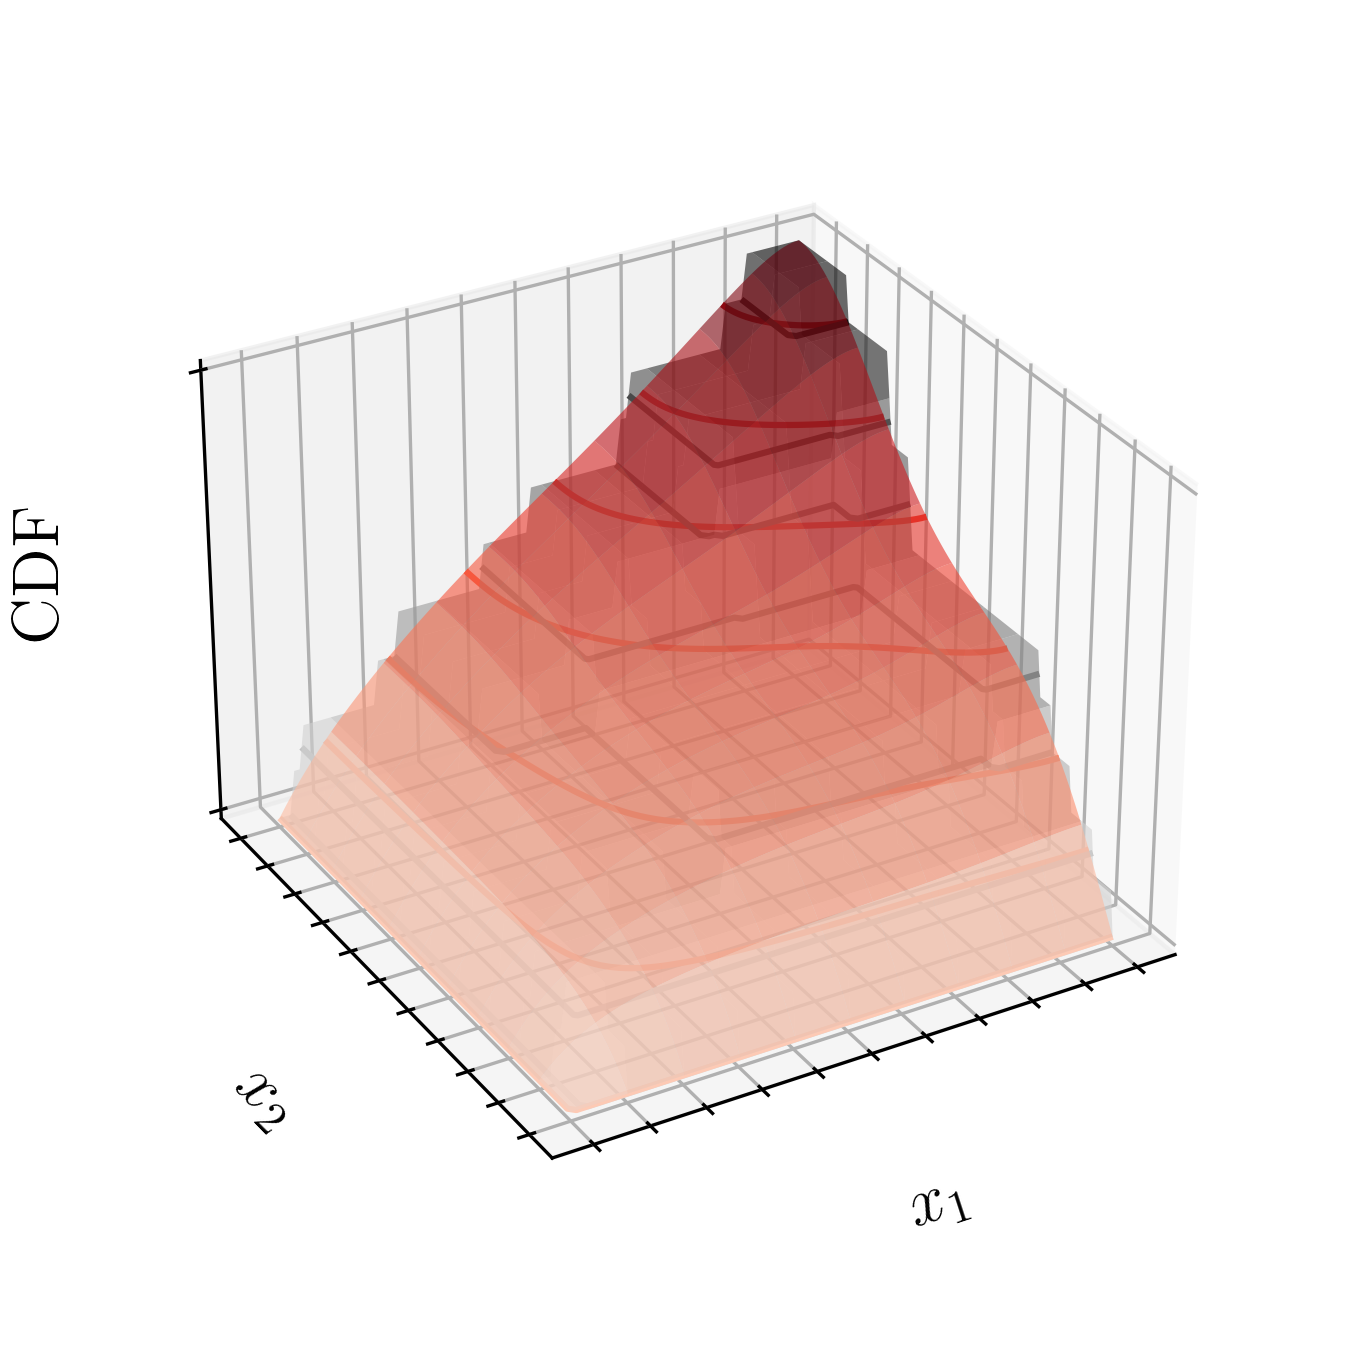
\includegraphics[width=\linewidth]{../numerical_experiments/chapter3/figures/ebc_m10.png}
        \caption{$B_{\bm}(C_n)$ with $(m_1=m_2=10)$.}
    \end{subfigure}
    \begin{subfigure}[b]{0.49\textwidth}
        \centering
        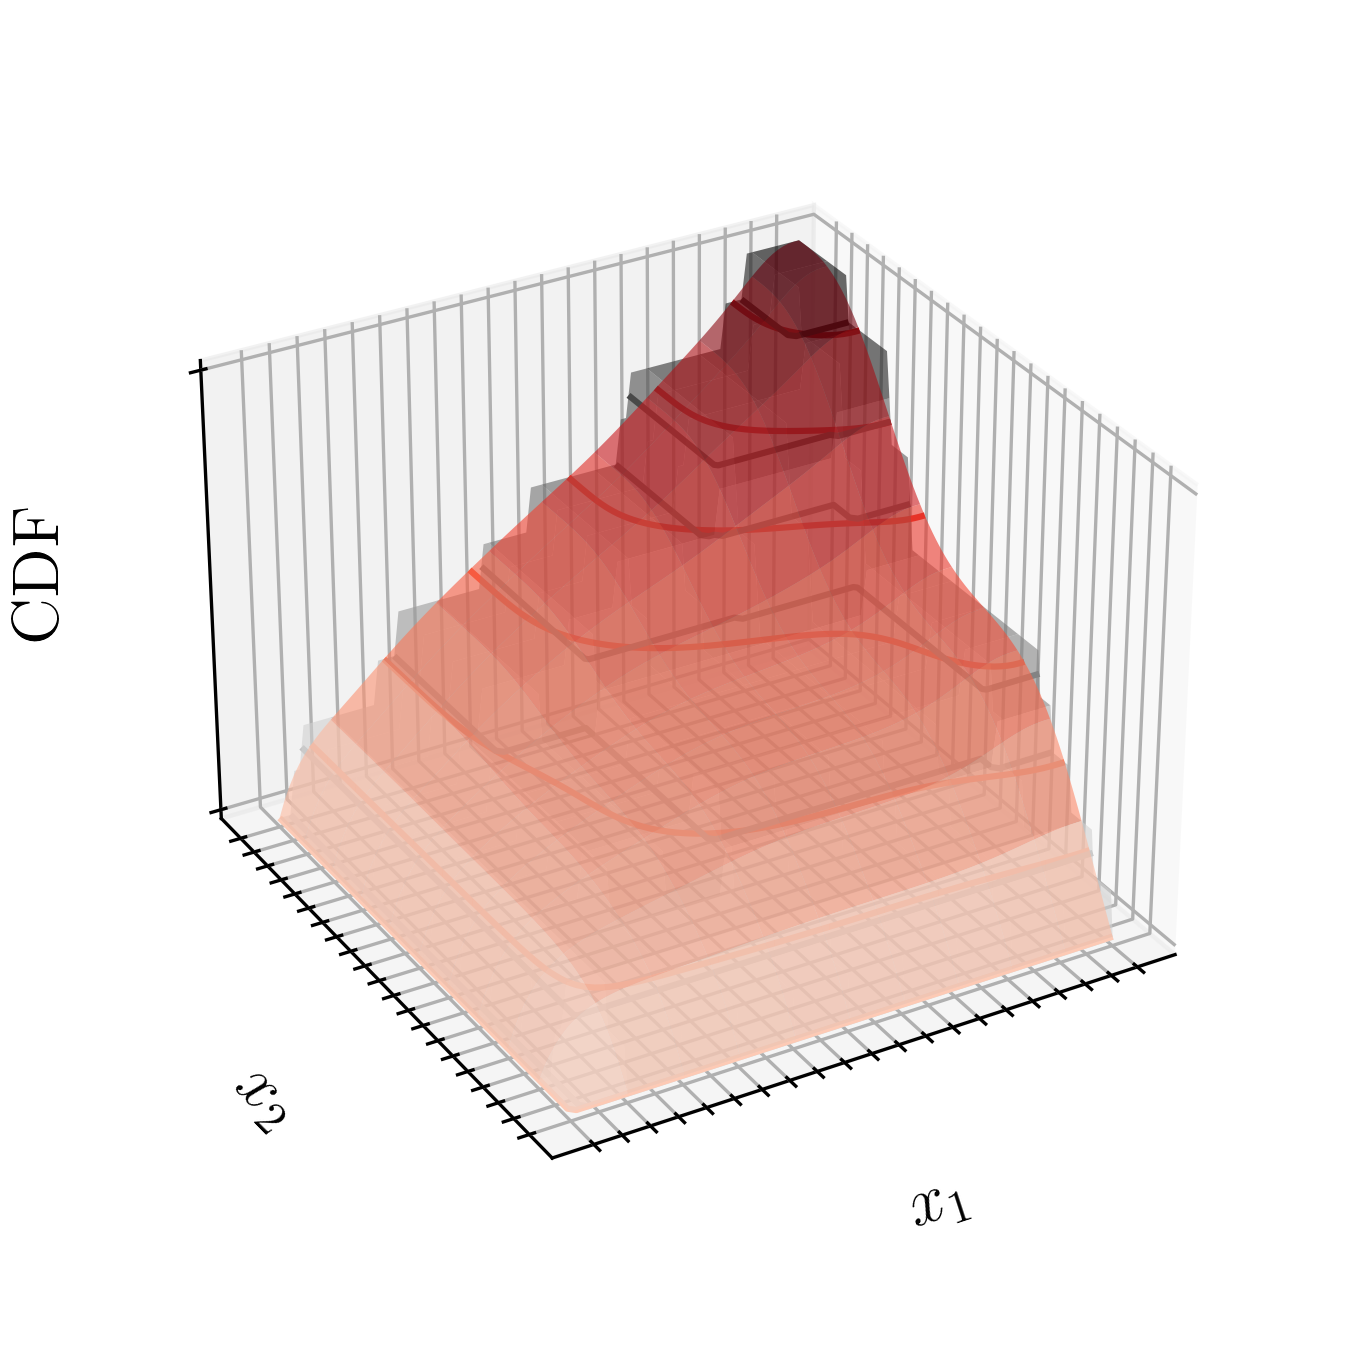
\includegraphics[width=\linewidth]{../numerical_experiments/chapter3/figures/ebc_m20.png}
        \caption{$B_{\bm}(C_n)$ with $(m_1=m_2=20)$.}
    \end{subfigure}
    \centering
    \caption{Bernstein approximations of the empirical copula $C_n$ (with size $n=10$) of a Clayton copula (with parameter $\theta=2.5$). The polynomial orders are assumed equal in the two dimensions $m_1=m_2\in\{3, 10, 20\}$.}
    \label{fig:ebc_illustration}
\end{figure}

\newpage
%============================================================%
%============================================================%
\section{\textit{Copulogram}: a tool for multivariate data visualization}\label{sec:copulogram}
%============================================================%
%============================================================%
In statistics, data visualization offers a wide set of tools to analyze data. 
Multivariate data visualization is of great help to apprehend problems with dimension higher than two. 
In the context of continuous variables, let us consider the $n$-sized sample $\bX_n = \left\{\bx^{(1)}, \dots, \bx^{(n)}\right\} \sim \bX \in \iD_{\bx}\subseteq\R^d$. 
The marginal samples of $\bX_n$ are denoted by $X_{n, j} = \{x_j^{(1)}, \dots, x_j^{(n)}\}, j\in \{1, \dots, d\}$.

Various techniques exist to represent multivariate data, such as the ``parallel coordinate plot'', also called ``cobweb plot'' (see e.g., \citep{heinrich_2013_cobweb}). 
For each sample $\bx^{(i)} \in \bX_n$, this plot draws a line passing by the values of $\bx^{(i)} = [x_1^{(i)}, \dots, x_d^{(i)}]$. 
This representation was used in sensitivity analysis to illustrate the connections between a set of inputs and an output, however, it does not provide a good representation of the dependence structure between the inputs. 

%============================================================%
\subsection{From pairwise plot to copulogram}
%============================================================%
Alternatively, the ``pairwise plot'', also named ``generalized draftsman plot'', was initially introduced by \citet{hartigan_1975_splom} to draw a matrix of scatter-plots between all the pairs of marginal samples $\{X_{n, i}, X_{n, j}\}, i \ne j \in \{1, \dots, d\}^2$. 
Because of the symmetry, the pairwise plot is usually represented on the lower triangle of the matrix. 
Later on, statisticians improved the pairwise plot by adding a histogram (or KDE) of the marginal samples $X_{n, j} j \in \{1, \dots, d\}$ on the diagonal. 
Additionally, the upper triangle was completed with the values of linear correlation for each pairs of marginal sample $\{X_{n, i}, X_{n, j}\}, i \ne j$. 
This matrix of correlation coefficients is also know as ``correlogram''. 
Altogether, this matrix plot became known as the ``scatter plot of matrices'' (SPLOM). 

However, the linear correlation coefficient is known to give a poor description of the dependence in nonlinear cases. 
When analysis a continuous sample $\bX_n \sim \bX$, the Sklar theorem states that the dependence structure within the random vector $\bX$ has a unique expression with its $d$-copula $C$. 
As mentioned in Section~\ref{sec:copula_prelims}, the component wise normalized ranks of the original sample $\bX_n$ define the empirical copula density $c_n$ (converging towards $C$ as $n$ increases).

To the best of our knowledge, the \textit{copulogram} is a new multivariate data visualization tool improving the SPLOM by representing the empirical copula density $c_n$ on the upper triangle of the matrix plot. 
This plot is an empirical decomposition of a multivariate sample in the vein of the Sklar theorem between marginals on the diagonal and copula on the upper triangle.

%============================================================%
\subsection{Implementation in a Python package}
%============================================================%

An open-source implementation is proposed in the python package \href{https://github.com/efekhari27/copulogram}{\texttt{copulogram}}. 
This code mostly relies on the Python package for data visualization \href{https://seaborn.pydata.org/}{\texttt{seaborn}} \citep{waskom_2021_seaborn}. 
The developments are tracked and archived in a GitHub repository\footnotemark and the package can be installed from the package-management system ``PyPI''. 

Multiple visual options are offered by the \texttt{copulogram} package, as illustrated in the GitHub repository. 
For example, the user can represent the univariate samples on the diagonal, or the bivariate samples in the triangles with kernel density estimation.  
Categorical variables can be used to assign different colors depending on the data class. 
The colors can also vary depending on a continuous variable after defining a mapping between the values of this variable and a set of color (also called colorbar).


\footnotetext{GitHub repository: \url{https://github.com/efekhari27/copulogram}}




\subsubsection{Example \#1: Iris flower dataset}
%------------------------------------------------------------%

The first example illustrates the copulogram on a widely used dataset in the machine learning community. 
The iris flower dataset was first introduced by Fisher and became a reference dataset for classification techniques. 
In the following lines of Python code, the dataset is loaded and the copulogram package is used to draw the new plot. 
The resulting copulogram applied to the iris flower data is represented in \fig{fig:iris_copulogram}. 
\lstset{style=mystyle, language=python}
%
\begin{lstlisting}
>>> import seaborn as sns
>>> import copulogram as cp

>>> data = sns.load_dataset("iris")
>>> copulogram = cp.Copulogram(data)
>>> copulogram.draw(hue="species")
\end{lstlisting}
%
Since this data mostly presents linear dependencies, the copulogram is not very instructive. 
In other cases, the role of the dependence in the joint distribution is more important.



\subsubsection{Example \#2: Ishigami function}
%------------------------------------------------------------%

The Ishigami function is commonly used as a benchmark problem for global sensitivity analysis (GSA): 
\begin{equation}
    y = g(x_1, x_2, x_3) = \sin(x_1) + 7 \, \sin(x_2)^2 + 0.1 \, x_3^4 * \sin(x_1).
\end{equation}
This uncertainty quantification problem considers an independent random input vector $\bX=\prod_{j=1}^{3} X_j$. 
While the marginals in GSA benchmarks are usually assumed to be uniform, they will be considered Gaussian hereafter to distinguish the different elements of the joint distribution. 
Therefore, let us define $X_j\sim \iN(0, 1) \forall j \in \{1, 2, 3\}$. 
In this setup, the random inputs are independent but they each present interesting dependencies with the random output $Y=g(\bX)$.

A Monte Carlo sample with size $n=10^3$ is generated, $\bX_n \simiid \bX$, and evaluated such that $Y_n=g(\bx_n)$.  
The copulogram of the input-output sample $(\bX_n, Y_n)$ is represented in \fig{fig:ishigami_copulogram}. 
As expected, the scatter-plots between the inputs in the upper triangle are uniform (representing an independent density copula). 

In GSA, the work of \citet{poczos_2012_copulaMMD} studied the discrepancy between the empirical density copula $c_n(X_j, Y), j \in \{1, \dots, d\}$ and the independent copula to qualitatively assess the importance of $X_j$.  
In the same vein, the paper of \citet{plischke_2019_copulaGSA} attempted to formalize a link between different GSA approaches based on copulas and to quantitative approaches as the Sobol' indices. 

\begin{figure}
    \centering
    \quad\qquad\qquad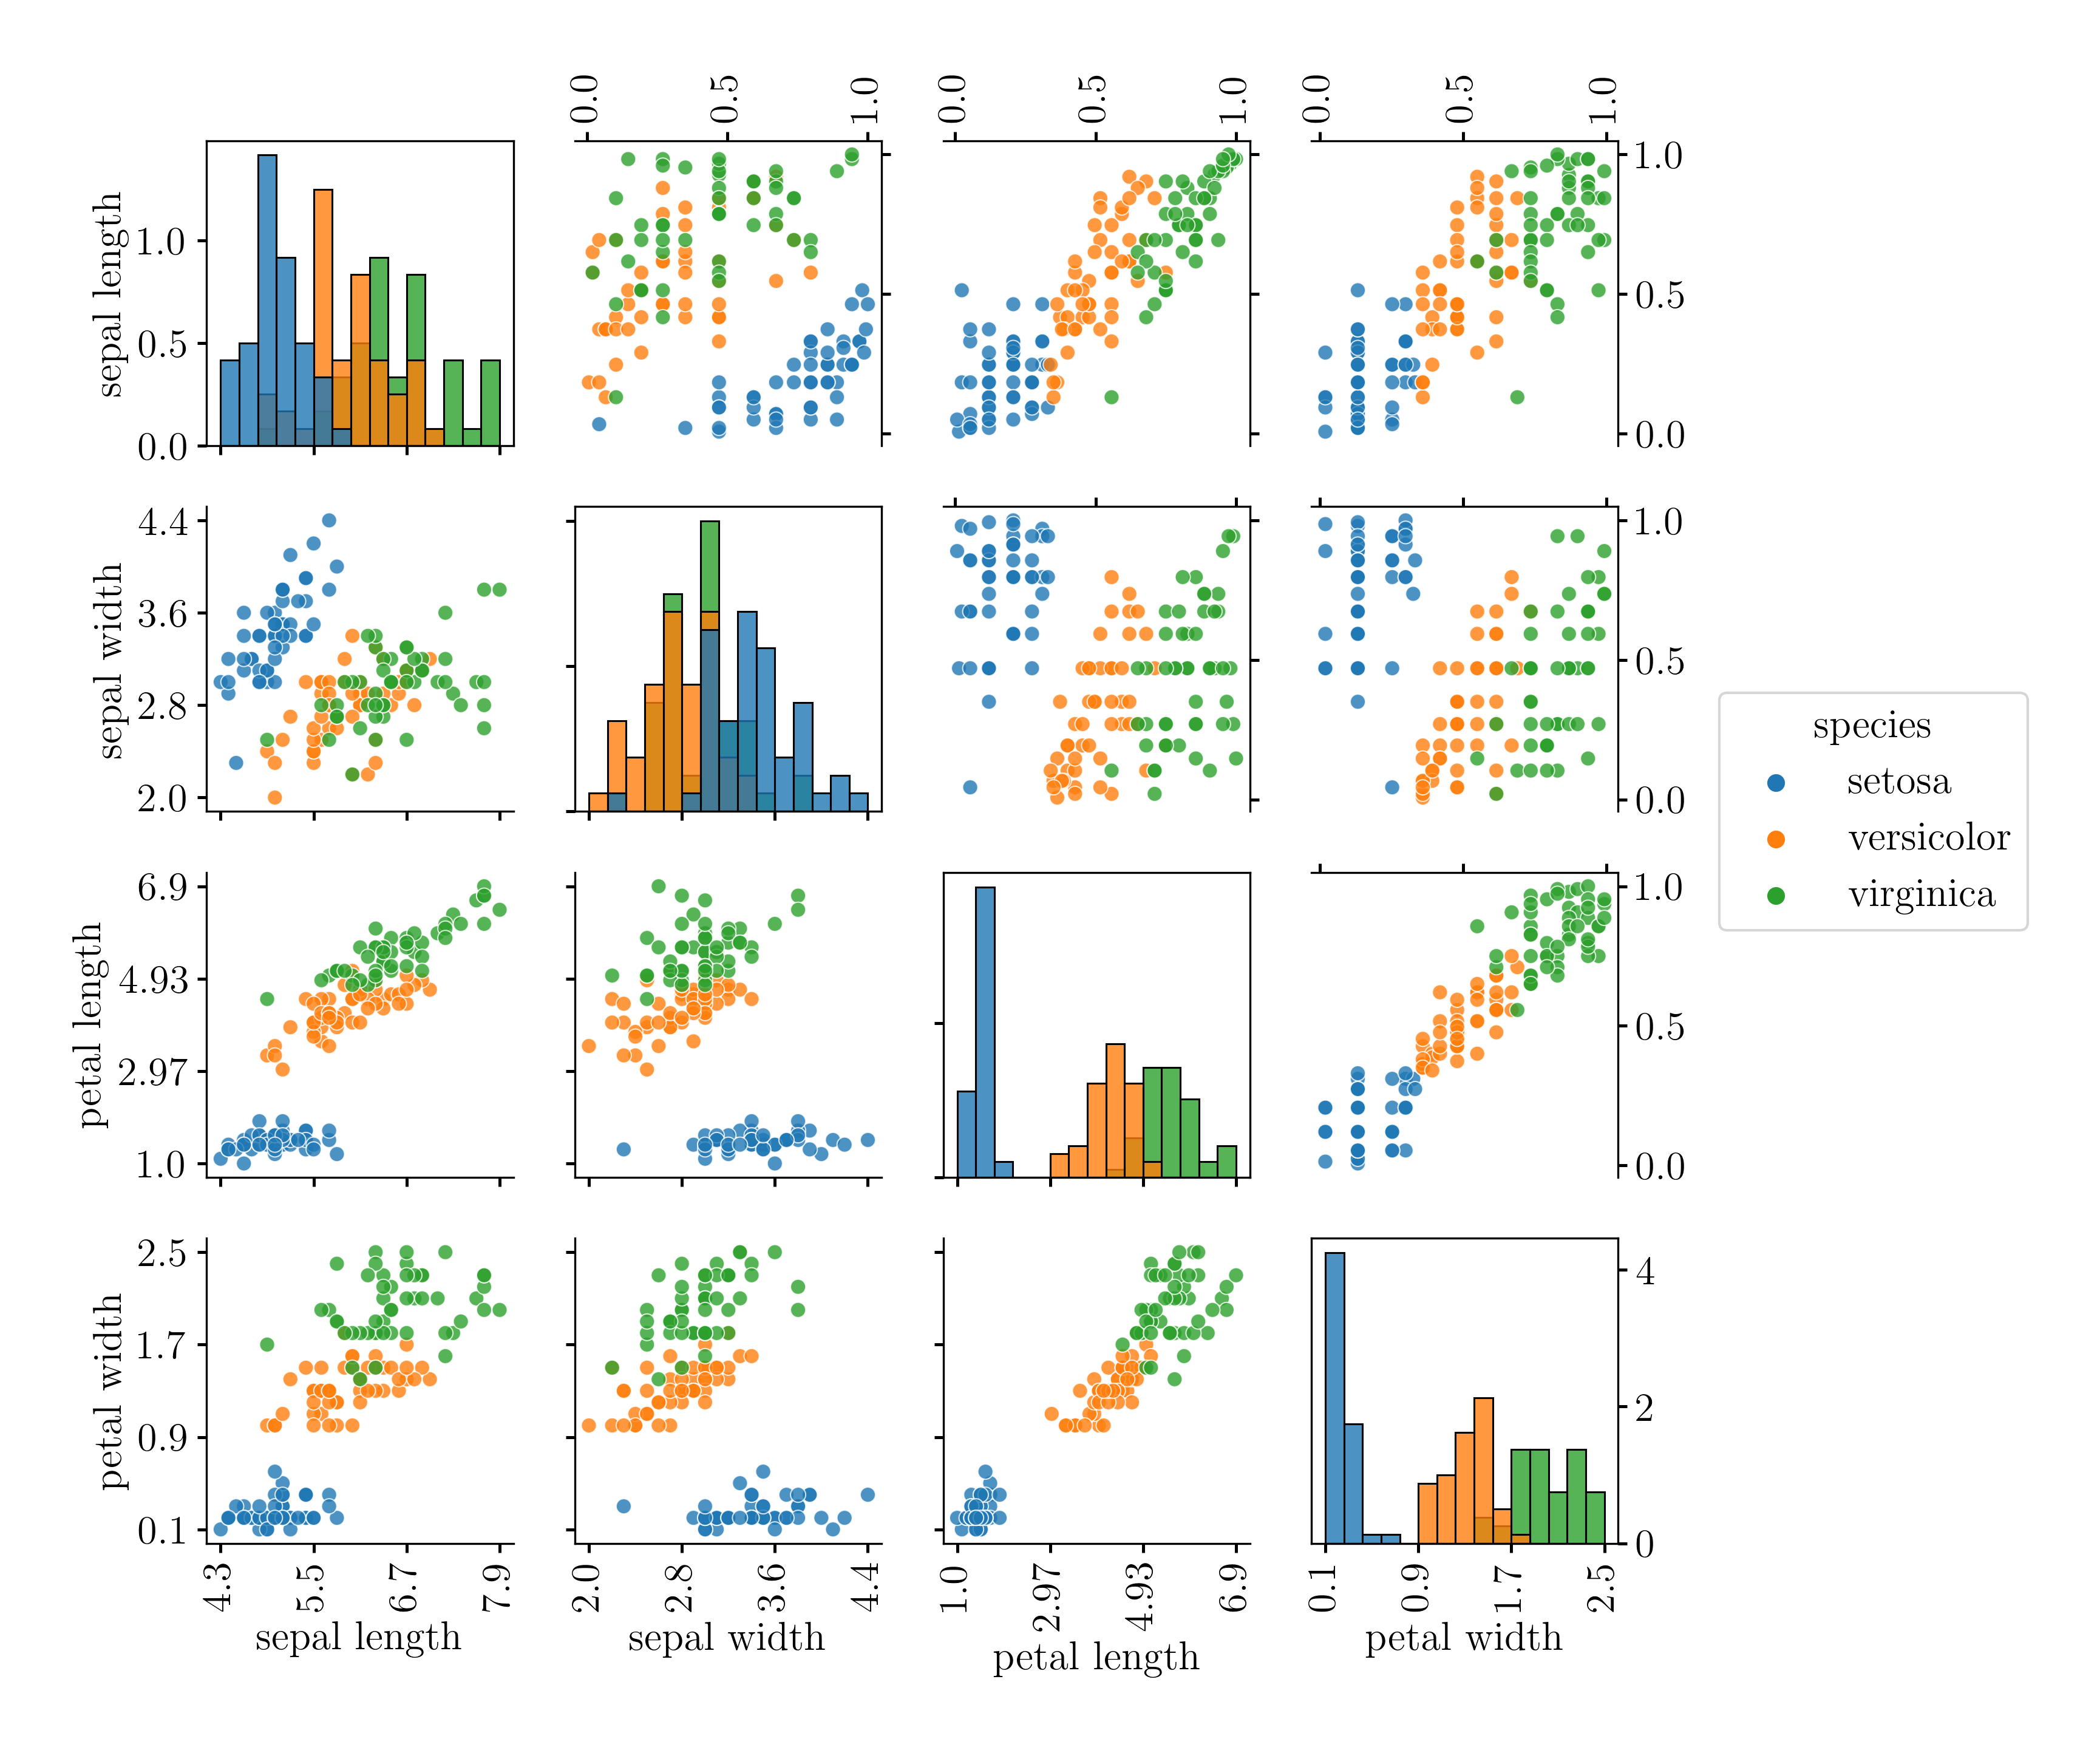
\includegraphics[width=0.82\textwidth]{../numerical_experiments/chapter3/figures/iris_copulogram.png}
    \caption{Copulogram of the iris flower dataset with colors assigned by the iris species.}
    \label{fig:iris_copulogram}
\end{figure}

\begin{figure}
    \centering
    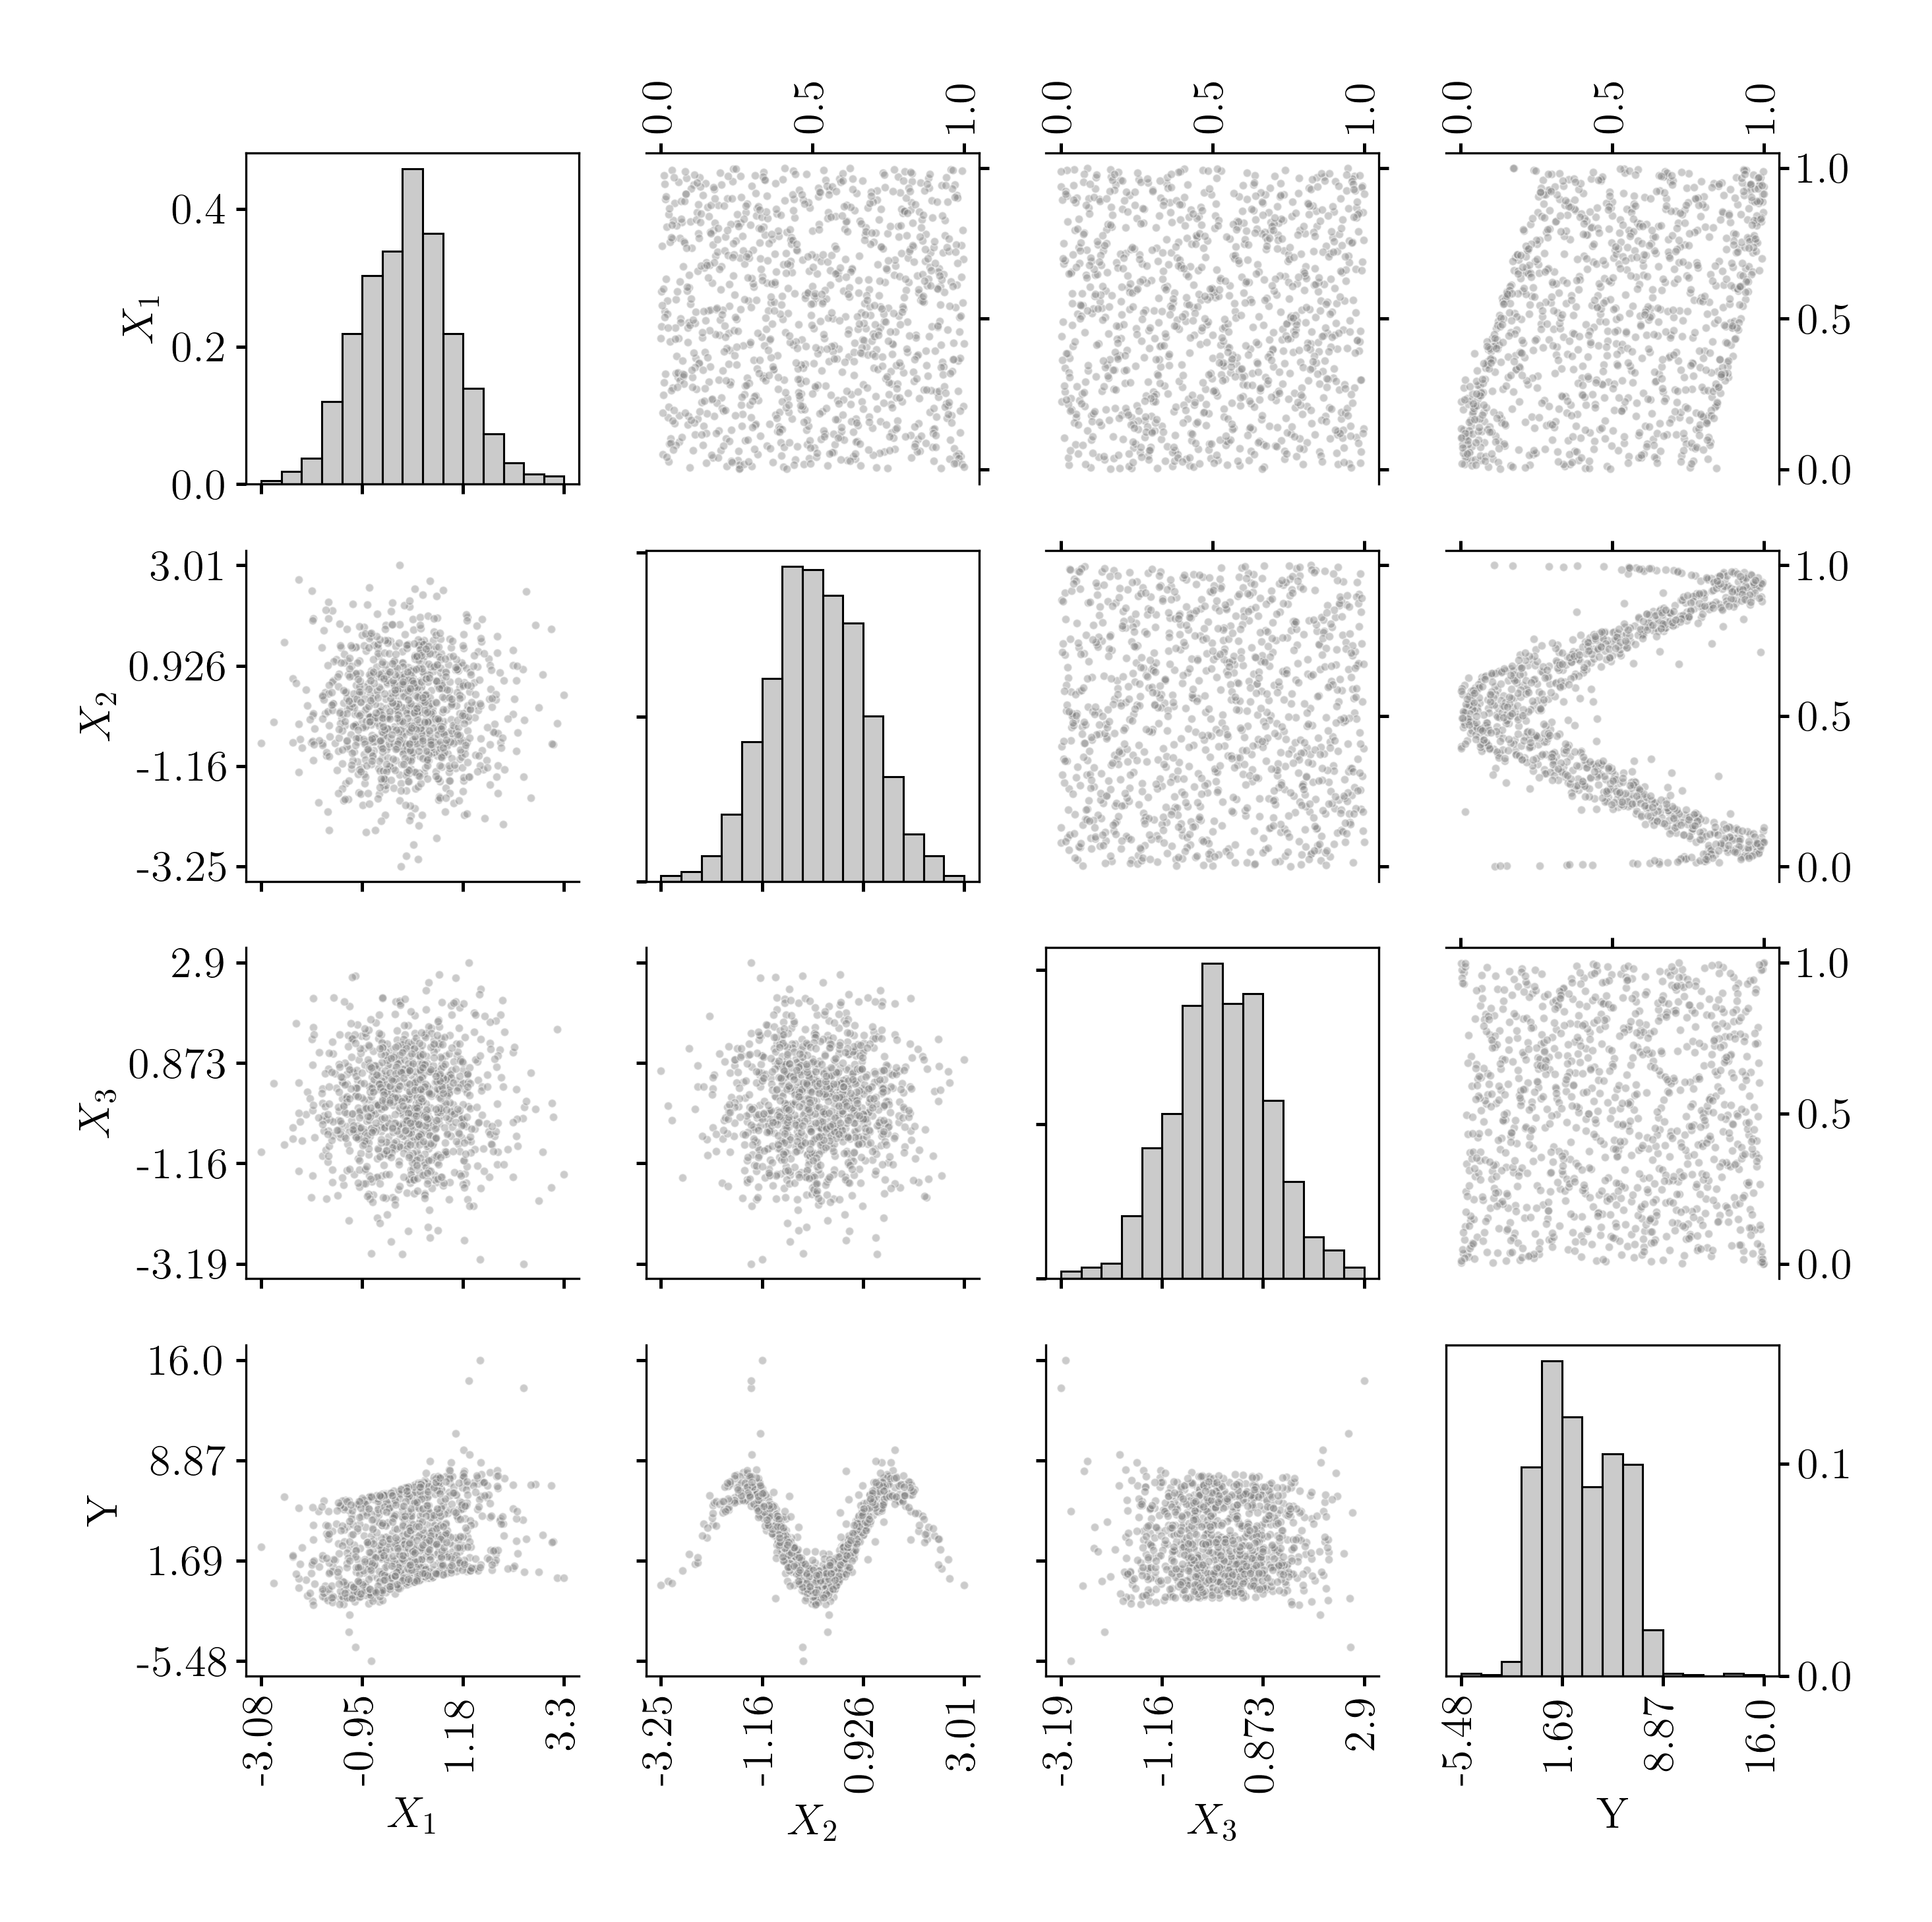
\includegraphics[width=0.7\textwidth]{../numerical_experiments/chapter3/figures/ishigami_copluogram.png}
    \caption{Copulogram of Monte Carlo sample (with size $n=10^3$) of the inputs and outputs of the modified Ishigami problem.}
    \label{fig:ishigami_copulogram}
\end{figure}



\newpage
%============================================================%
%============================================================%
\section{Semiparametric inference of the South Brittany metocean conditions} \label{sec:32_inference}
%============================================================%
%============================================================%

\elias{When should we use nonparametric copula inference? }

\citet{joe_2014}, p.250 discusses the use of nonparametric methods for multivariate inference. 
According to the author, 

``Non-parametric estimation of a copula is desirable if univariate margins are well-behaved and can be fit with parametric families, 
and the multivariate dependence structure is more complex than monotone relations among variables. 
If the univariate margins are also not simple, then multivariate non-parametric estimation approaches can be applied to the multivariate distribution directly, 
rather than estimation of non-parametric univariate margins with a non-parametric copula.
''

\begin{itemize}
    \item There is a difference between inference for central tendency study or extreme value theory. 
    \item In the present work, the focus is on complex dependence modelling
    \item 
\end{itemize}

\elias{Conditional model to infer the dependence: present how it looks and the difficulty to define it.}

\elias{If Alexis scripts work: compare the adequancy between the two strategies using the MMD for increasing sample sizes. }


%============================================================%
\subsection{Parametric marginal inference}
%============================================================%



%============================================================%
\subsection{Nonparametric Bernstein copula inference}
%============================================================%



%============================================================%
\subsection{Goodness-of-fit and discussion}
%============================================================%



\newpage
%============================================================%
%============================================================%
\section{Quantifying and clustering the wake-induced perturbations within a wind farm}
%============================================================%
%============================================================%
\elias{add ref: ``Difference in load predictions obtained with effective
turbulence vs. a dynamic wake meandering
modeling approach''}


In the offshore wind industry, the wake effect is considered crucial for electricity production and structural fatigue of turbine components. 
For instance, the standards developed by the International Electrotechnical Commission (see appendix E in \cite{IEC61400-1}) review some analytical \cite{Frandsen2007}, and numerical models (e.g., the dynamic wake meandering approach by \cite{Larsen2008}) to simulate the wind speed deficit and the wake added turbulence. 
Since the pioneering work of \cite{Jensen1983}, several wake models were developed and compared in a benchmark by \cite{Doubrawa2020}. 
This work takes advantage of the low computational cost of steady-state wake models to propagate the uncertainty from ambient to wake-induced wind conditions seen on a farm. 
It is worth noting that the wake creates a heterogeneous wind field in a wind farm, resulting in different loading conditions which should be considered at the stage of reliability based design (RBD). 
Such heterogeneity is not taken into account by the design load cases of international standards (see e.g., \cite{IEC61400-1,DNV-OS-J103}) where wind and wave conditions are derived from scenarios occurring over long-term periods. 
Wake models allow us to simulate the wind conditions' distribution at each turbine, however, the RBD step is too costly to be performed for each turbine. 
For further details regarding the RBD, one may refer to the work of \cite{huchet_2019, slot_sorensen_2020, stieng_muskulus_2020, wilkie_galasso_2021}, proposing several approaches to reduce the computational cost of this step. 
In order to speed up the RBD at the scale of a wind farm, the present work aims at building clusters of WT similarly affected by the wake. 
Then, the RBD over a wind farm can be computed only on a few WT, each representing a cluster of turbines enduring similar wake-modified wind loading. This clustering is done on two wind parameters, following the conclusions of the global sensitivity analysis of \cite{McWilliam2022}. 
In order to discriminate the wake-perturbed distributions of wind parameters, the maximum mean discrepancy (MMD) is used as a statistical metric between multivariate distributions (as reviewed by \cite{Sriperumbudur2010}). 
To illustrate this novel approach, a theoretical wind farm for the ongoing tenders off the coast of South Brittany in France is studied, with a modified version of the floating offshore wind turbine (FOWT) IEA-15MW (initially proposed in \cite{Allen2020,Gaertner2020}). 
Figure~\ref{fig:SB-farm} illustrates the layout of the 25 FOWT considered in the following. 
This layout is regular with an inter-turbine distance of seven times the rotor diameter in the dominant wind direction and five times the rotor diameter in the orthogonal (crosswind) direction. 
More details regarding the FOWT modifications and theoretical wind farm can be found in \cite{Capaldo2021,Peyrard2022}.

\begin{figure}[h]
\centering
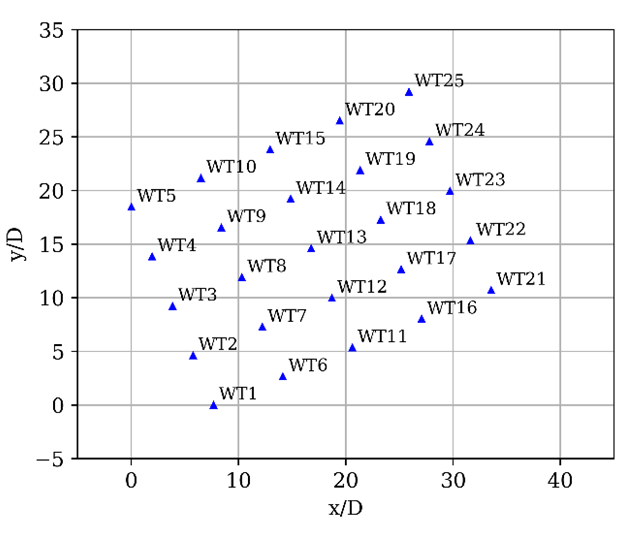
\includegraphics[width=15pc]{part2/figures/WAKE/SB1.png}
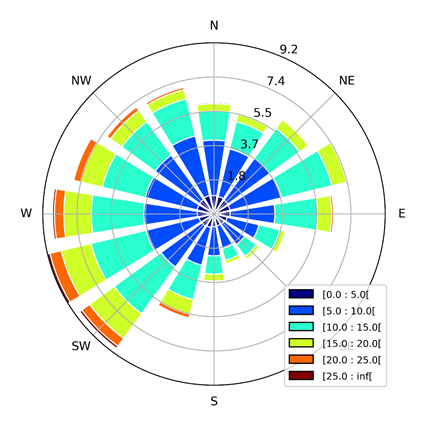
\includegraphics[width=13pc]{part2/figures/WAKE/SB2.png}\hspace{2pc}
\caption{\label{fig:SB-farm} 
South Brittany wind farm layout (left). South Brittany wind rose from the ANEMOC data (right, source: \cite{Ardillon2023}).}
\end{figure}

Based on the results of previous numerical studies, with either dynamic wake meandering \cite{Wise2020} or LES \cite{Johlas2021}, we retain the time-averaged floater position (translation and rotation) as the main effect of the floater motion on the far wake. It was shown that this effect is small, both on the wake-added turbulence and on the wind speed deficit. However, noticeable uplift of the wake may influence the fatigue design. 

The key idea in this paper to reduce the number of cases for RBD is to employ clustering techniques on the wake-induced wind parameters, to constitute groups of WT that are exposed to similar design load conditions. To do so, the present work is divided into four sections. First, the wake model used in this work is presented in section~\ref{sec:farmshadow}. Then, section~\ref{sec:UQ-wake} describes the uncertainty propagation through the wake model, from the probabilistic distribution of ambient wind parameters to the wake-modified wind parameters distribution within the farm. In order to regroup the similar wake-modified distributions, an adapted statistical metric on multivariate distributions is introduced in section~\ref{sec:metric}. Finally, the application of several clustering methods to the South Brittany case study is compared in section~\ref{sec:clustering}. The main conclusion suggests four clusters among the 25 FOWT which can then be used for RBD analysis of the farm.


%============================================================%
\subsection{Uncertainty propagation in a wake model}\label{sec:UQ-wake}
%============================================================%
The wake model described in section~\ref{sec:farmshadow} takes as input a set of variables describing the ambient wind conditions $\bx \in \mathbb{R}^3$ and computes the perturbed wind conditions at each WT represented by the vector $\bx _l', l \in (1,..,n_{WT})$, where $n_{WT}$ is the total number of turbines in the farm:
\begin{align}
    g:\mathbb{R}^3 &\rightarrow \mathbb{R}^{3 n_{WT}} \\
    \bx &\longmapsto g(\bx) = (\bx_1',..,\bx_{n_{WT}}')
\end{align}
The uncertainties associated with the ambient wind conditions are represented by a random vector $\bX$ following the distribution $p_0$. 
Note that the index 0 is a reference to the fact that these conditions are not perturbed by the wake. 
A parametric model has been fitted in \cite{vanem_fekhari_2023} using conditional probability density functions to capture the dependence structure, with an approach similar to the one presented in~\cite{kelly_2022}. 
The random vector $\bX$ is described by the following input random variables:
\begin{itemize}
    \item Mean wind speed ($u$) is the 10-min average horizontal wind speed at hub height.
    \item Wind turbulence intensity ($TI$) is the 10-min wind speed turbulence intensity at hub height.
    \item Wind direction ($\theta$) is the 10-min average wind direction.
\end{itemize}
In the following, we assume the wind orientation variable $\theta$ to be unaffected by the wake. 
When perturbed by the wake of the wind farm, the WT~$l$ sees a wind flow represented by the random vector $\bX_l',l \in (1,..,n_{WT})$, following the distribution $p_l'$. 
Then, the two remaining parameters are $u_{rotor}$ and $TI_{rotor}$ to represent this modified wind flow on a vertical plane located at each WT. 
These two quantities of interest are averaged over the rotor while the input parameters are given at hub height. For the sake of simplicity, we will neglect this difference in what follows in order to consider the transformation $\bX'=g(\bX)$ as a simple perturbation of $\bX$. We will abusively denote $u$ and $TI$ both the input and output quantities. 
The output of the uncertainty propagation is a set of perturbed environmental distributions $p_l',l \in (1,..,n_{WT})$.
A Monte-Carlo sample $\bX_n={\bx^{(1)},..,\bx^{(n)}}$ of the three random input variables is generated. 
Then, considering the farm layout illustrated in Figure~\ref{fig:SB-farm} and a constant wind shear exponent of 0.1 like in section~\ref{sec:farmshadow}, a wake simulation is run for every wind condition of the Monte Carlo design of experiments. 
The code output consists in a multivariate joint distribution of modified $u$ and $TI$ for each WT. As the Monte Carlo procedure is known to converge slowly but surely, it was chosen to perform this uncertainty propagation with a number of simulations of size $n=6~000$ because of its simplicity and the low computational cost of the simulations.

 We can plot a preview of the wake perturbations on the joint distribution for given WT in the two dimensions $u$ and $TI$. 
 Figure~\ref{fig:FIGJointPerturbationSB} illustrates this perturbation for three WT differently affected by the wake depending on their position in the farm (cf. Figure~\ref{fig:SB-farm}). 
 One can notice that the WT~25 distribution (in orange) is very close to the ambient distribution (in black), as expected, this WT being located on the edge of the farm and facing the dominant wind direction. 
 Meanwhile, the WT~13 distribution (in red) seems more affected by the wake, by getting a higher wind turbulence with lower wind speed. 
 This analysis can be completed with the two marginals in Figure~\ref{FIGMarginalWSP} and Figure~\ref{FIGMarginalTI}, both describing the ambient marginal distributions (in black) and wake-disturbed distributions. 
 In general, a small wind speed deficit is noticed as indicated by the small shifts of the probability density functions to the left on Figure~\ref{FIGMarginalWSP}. 
 Also, a small added turbulence is indicated by the small shifts of the curves to the right on Figure~\ref{FIGMarginalTI}. 
 Ideally, a tool should allow us to quantify the perturbation between the ambient and perturbed distributions.

\begin{figure}
    \centering
    \begin{subfigure}[b]{0.3\textwidth}
        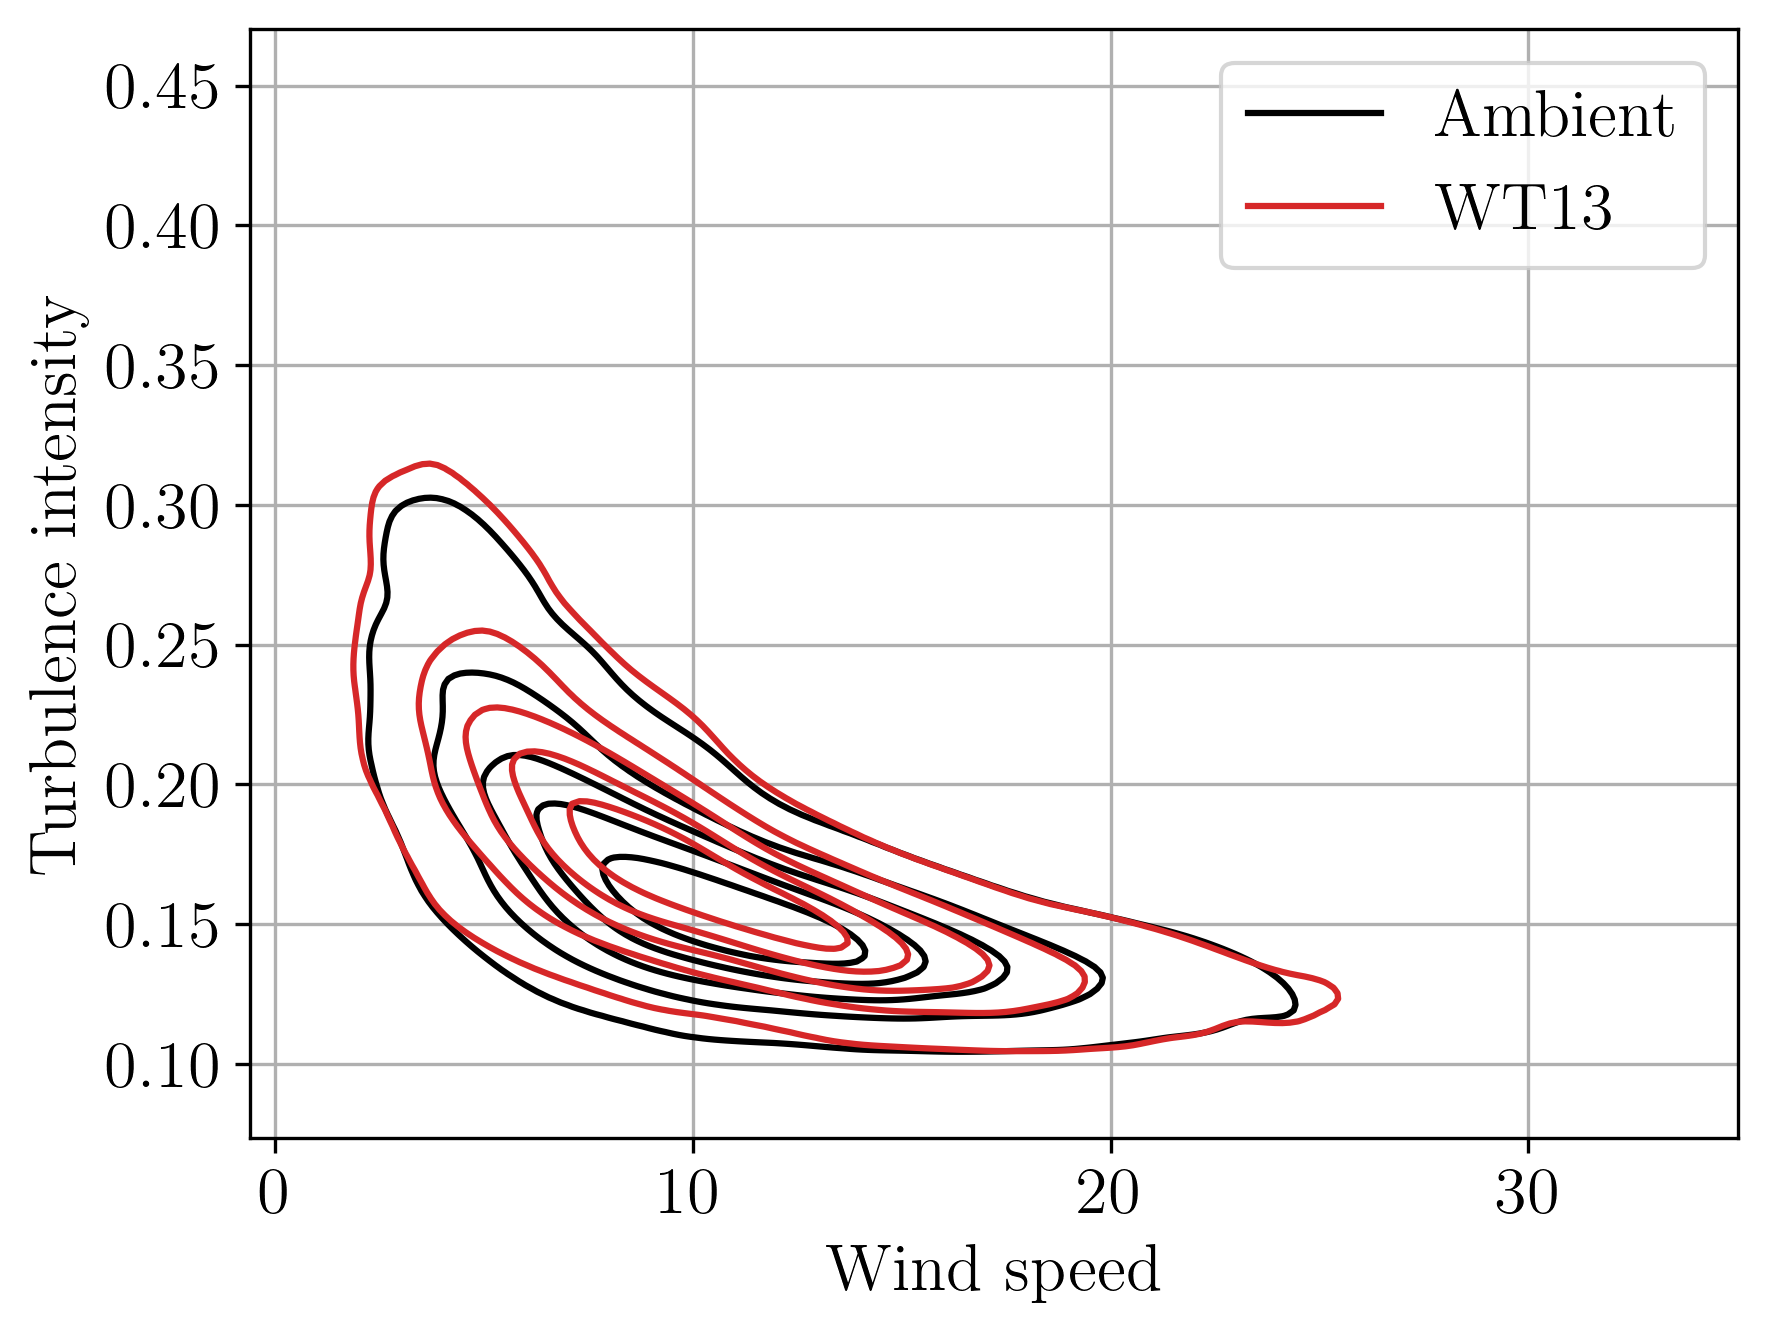
\includegraphics[width=\textwidth]{part2/figures/WAKE/joint_perturbation_SB_WT13.png}
    \end{subfigure}
    \begin{subfigure}[b]{0.3\textwidth}
        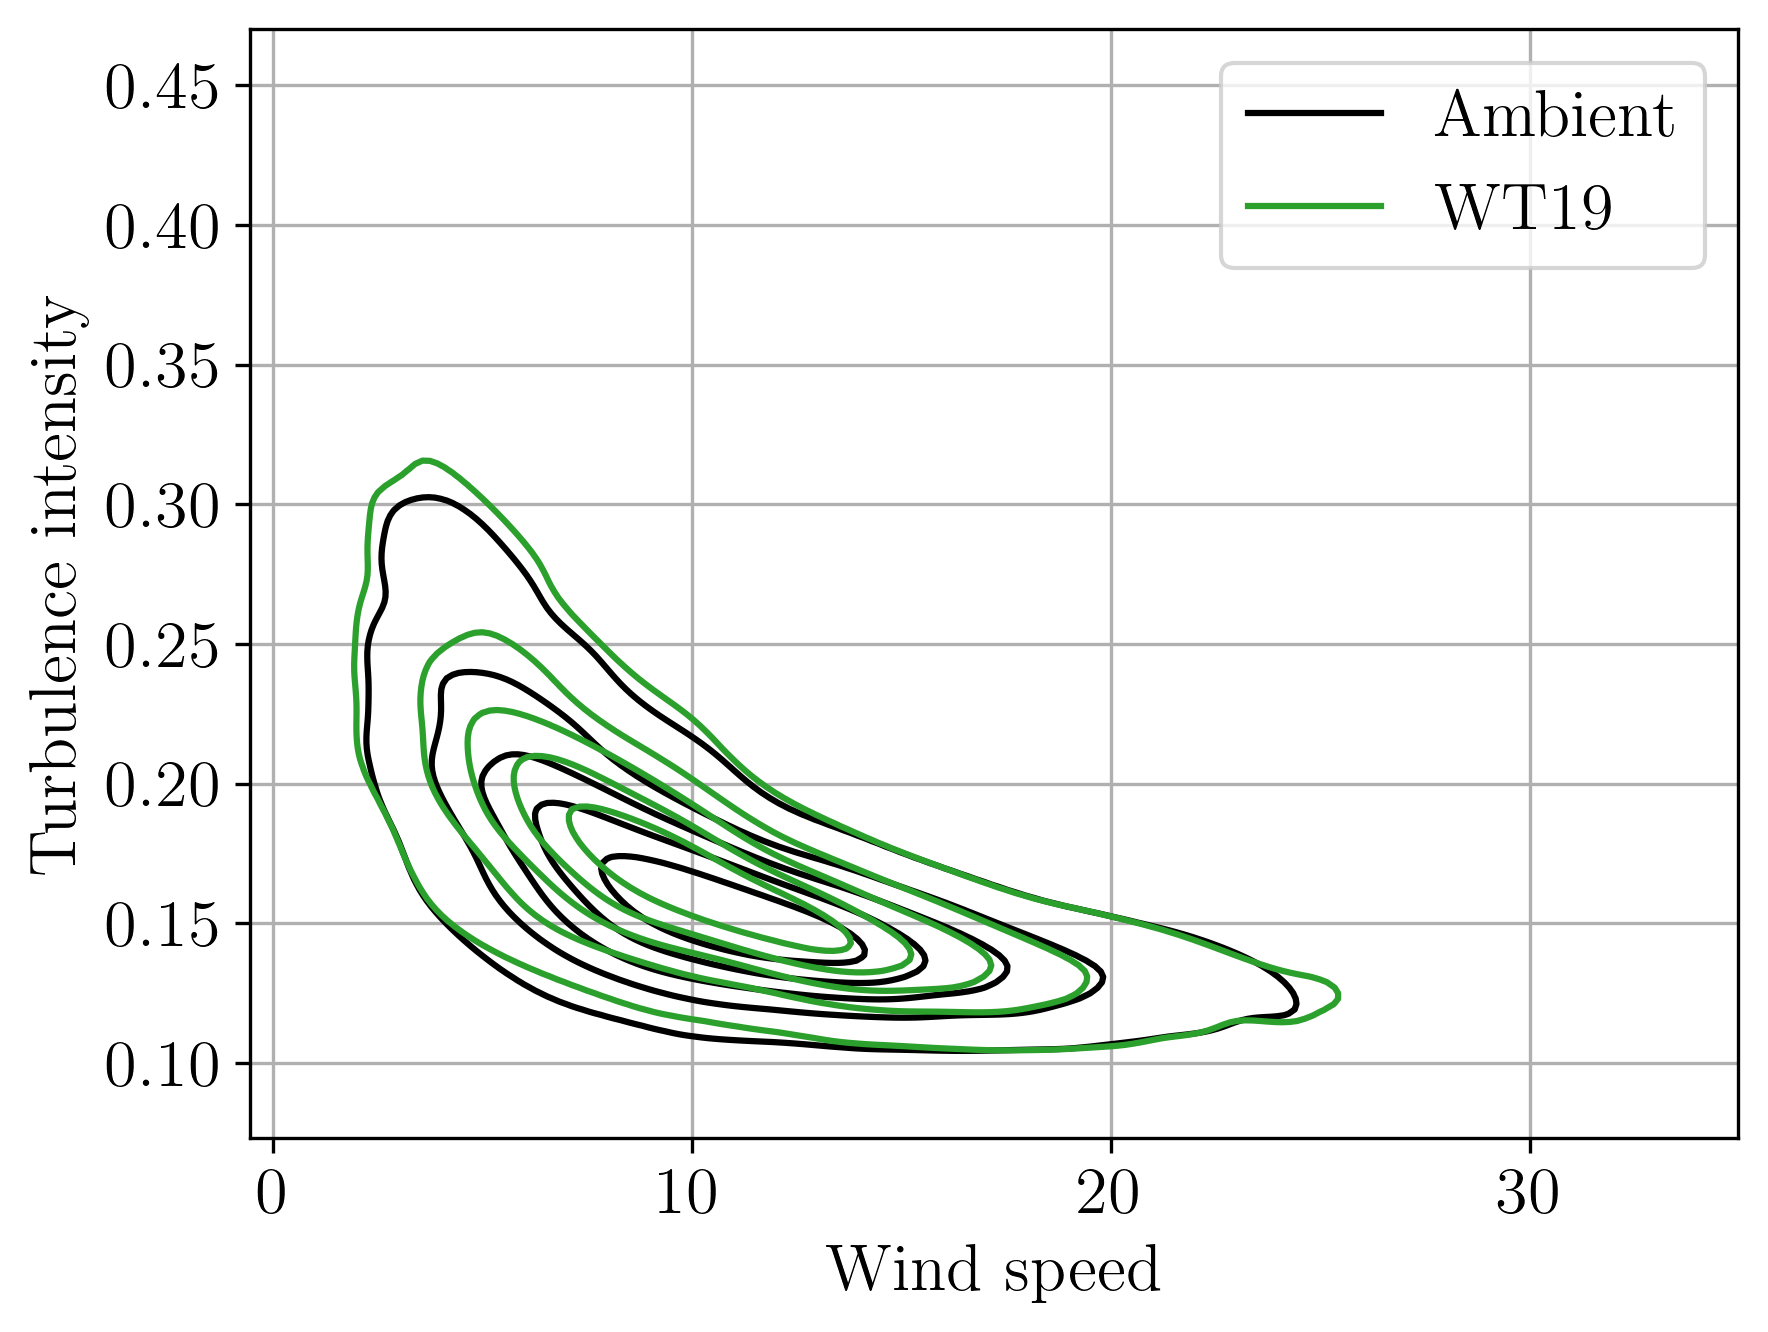
\includegraphics[width=\textwidth]{part2/figures/WAKE/joint_perturbation_SB_WT19.png}
    \end{subfigure}
    \begin{subfigure}[b]{0.3\textwidth}
        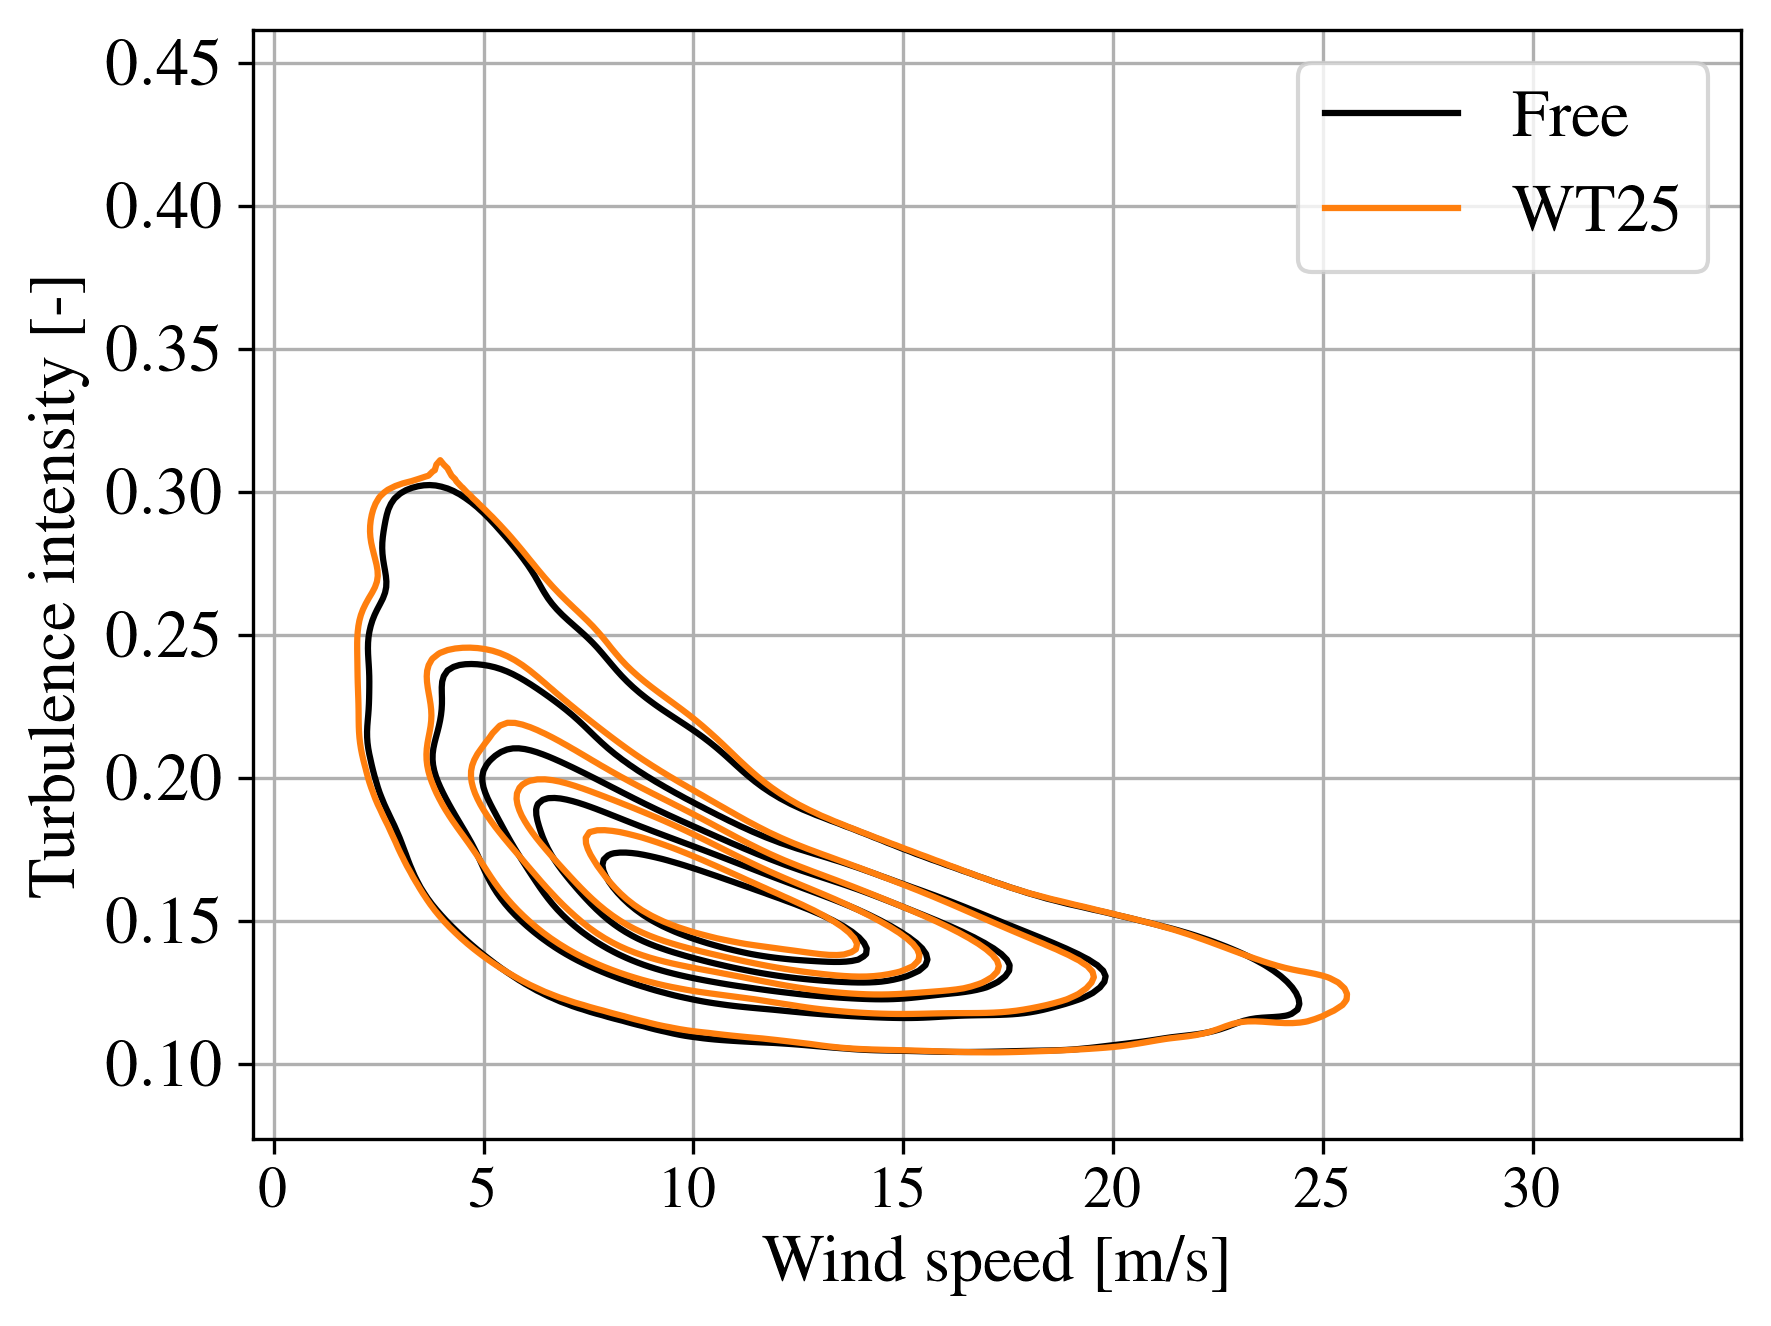
\includegraphics[width=\textwidth]{part2/figures/WAKE/joint_perturbation_SB_WT25.png}
    \end{subfigure}
    \caption{Joint perturbation at WT 13, 19, and 25}
\label{fig:FIGJointPerturbationSB}
\end{figure}

\begin{figure}
    \centering
    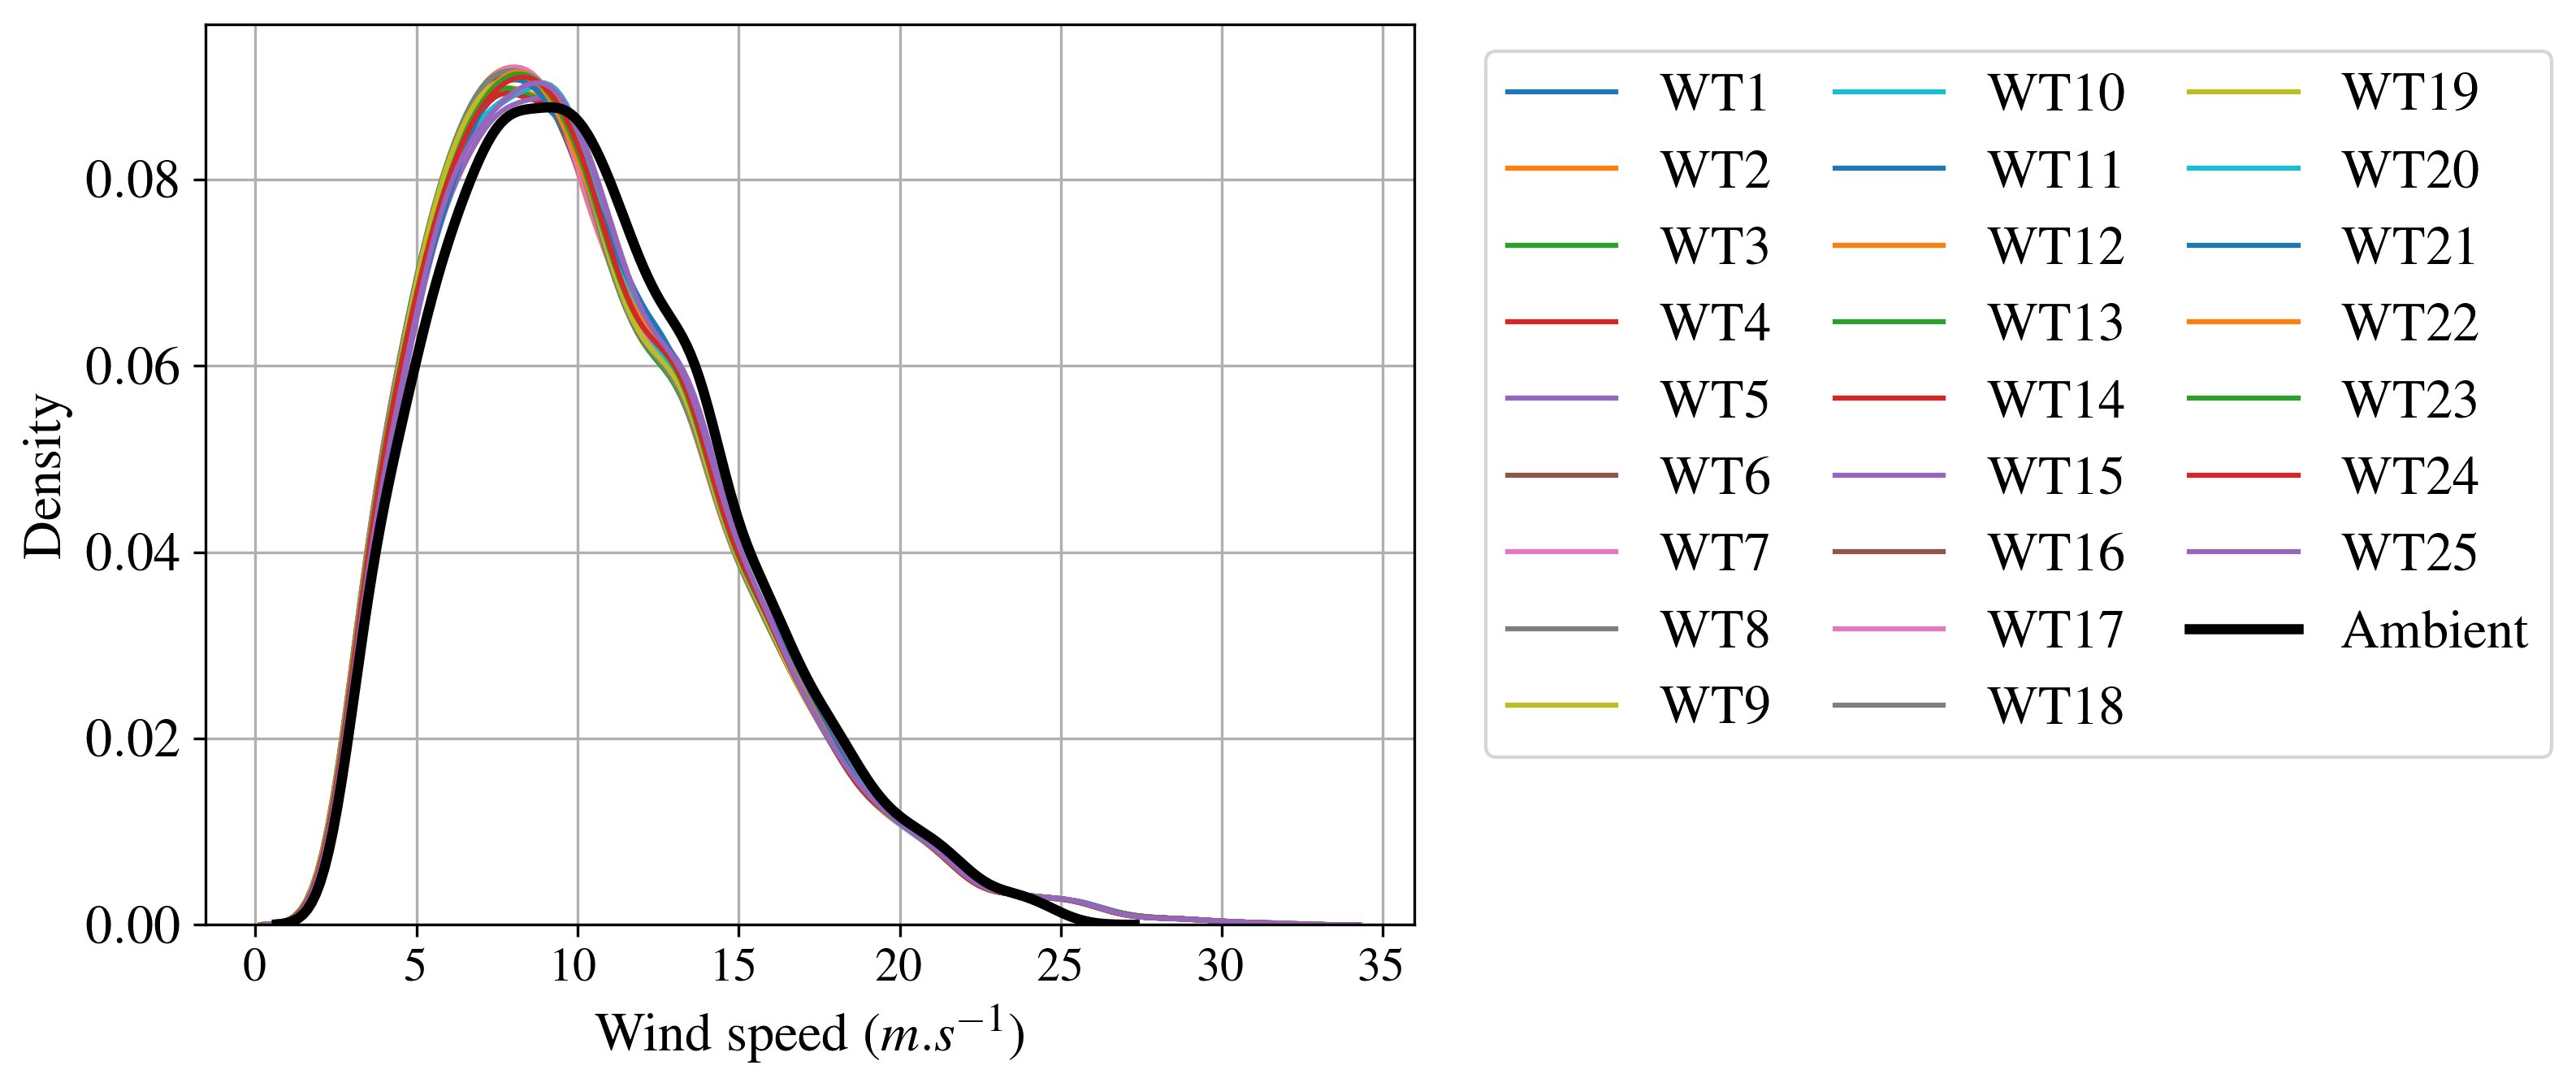
\includegraphics[width=0.7\textwidth]{part2/figures/WAKE/perturbed_wsp_distribution_SB.png}
    \caption{Ambient and wake-disturbed distributions of the wind speed}
\label{FIGMarginalWSP}
\end{figure}

\begin{figure}
    \centering
    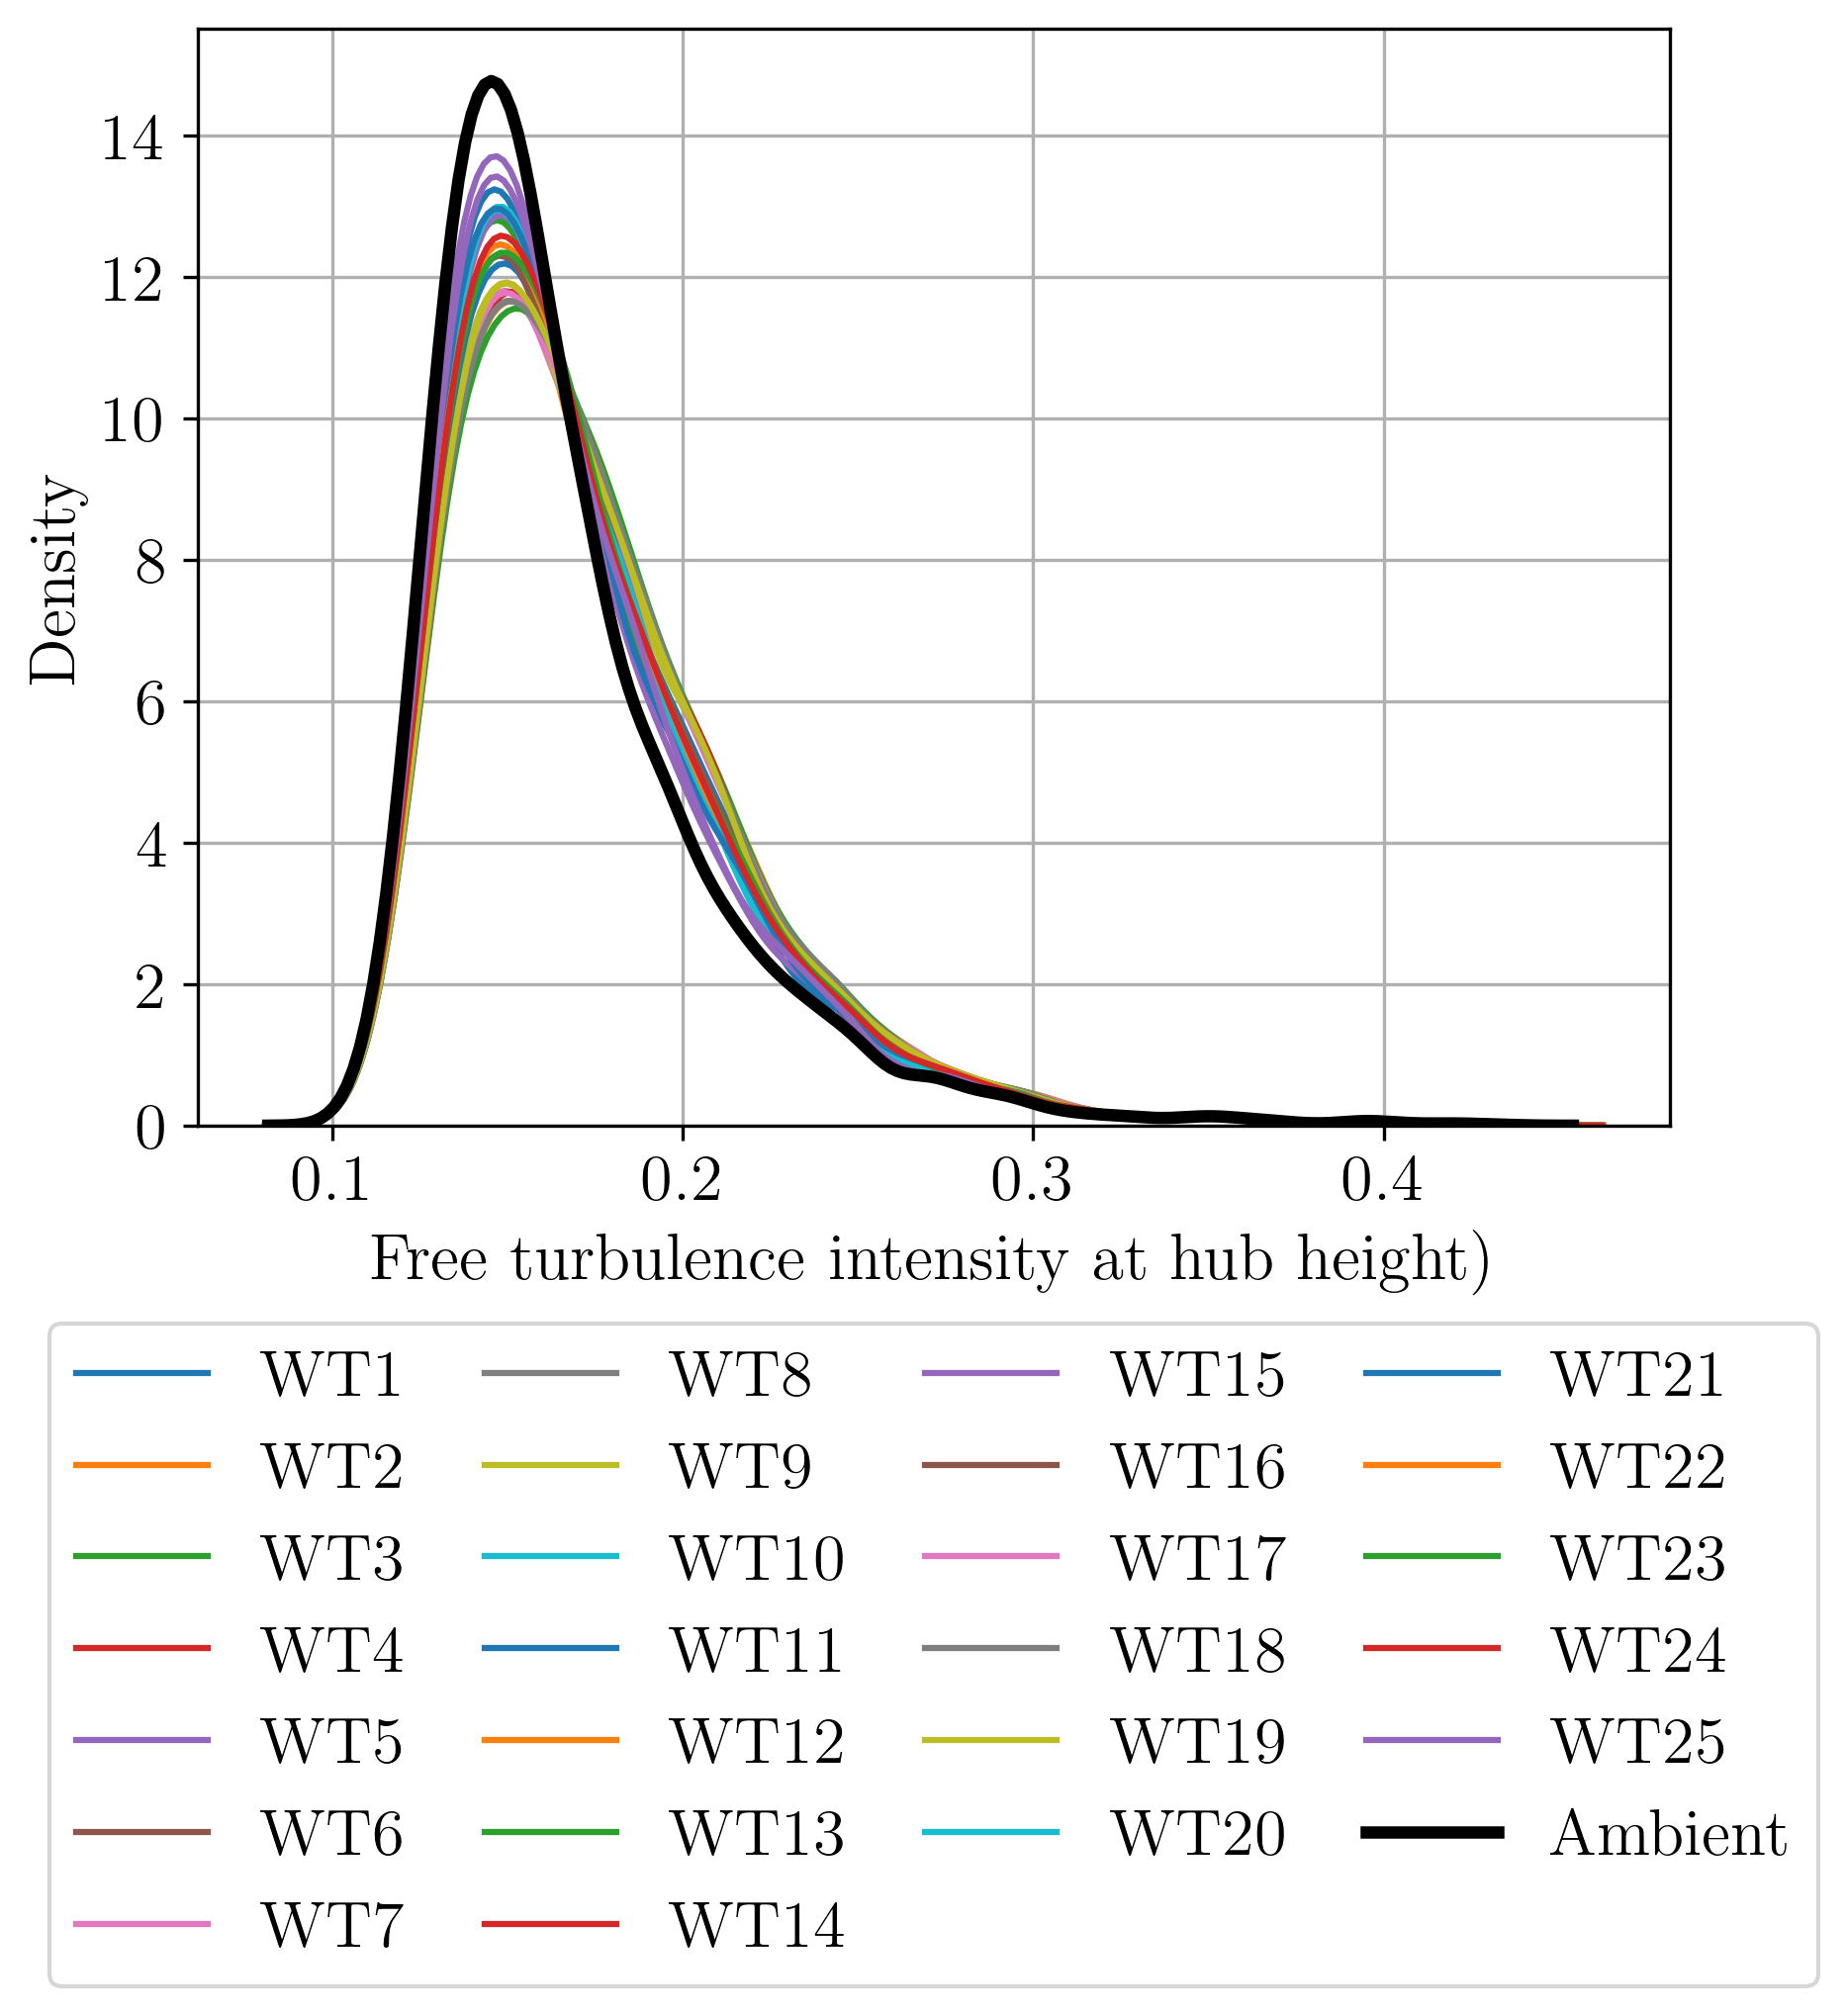
\includegraphics[width=0.7\textwidth]{part2/figures/WAKE/perturbed_ti_distribution_SB.png}
    \caption{Ambient and wake-disturbed distributions of the turbulence intensity}
\label{FIGMarginalTI}
\end{figure}




%============================================================%
\subsection{Statistical metric of wake-induced perturbations}\label{sec:metric}
%============================================================%

%------------------------------------------------------------%
\paragraph{Maximum mean discrepancy: a distance between distributions}
%------------------------------------------------------------%
In the literature, the maximum mean discrepancy was introduced by \cite{gretton_2006} as a statistical test to discriminate two distinct distributions. 
After further work on this tool, authors such as \cite{sriperumbudur_2010} showed that the MMD is a distance between two distributions embedded in a specific function space. 
Therefore, this concept relies on the embedding of distributions in a convenient Hilbert space.
Considering a positive-definite kernel $k:\mathbb{R}^d \times \mathbb{R}^d \xrightarrow{} \mathbb{R},d \in \mathbb{N}$ 
generating a unique Hilbert space $\iH_k$ of functions equipped with inner products $ <\cdot,\cdot >_{\iH_k}$ and norms $\| \cdot \| _{\iH_k}$ (also called Reproducing Kernel Hilbert 
Space (RKHS) when the function $k(\bx,\cdot )$ satisfies the reproducing property). 
Then, let us define the kernel mean embedding of the distribution $P$ in the function space $\iH_k$:
\begin{equation}
\mu_P (\bx):=\int_{\mathbb{R}^d}{k(\bx, \by) \mathrm{d}P(\by) } \approx \frac{1}{n} \sum_{i=1}^{n}{k(\bx,\bx^{(i)})},\, \bx^{(i)} \in \bX_n.
\end{equation}
The kernel mean embedding is approximated on sample $\bX_n=(\bx^{(1)},..,\bx^{(n)})$ following the distribution $P$.
Figure \ref{fig:kernel_embedding} illustrates the kernel mean embedding of two distributions in the function space $\iH_k$ defined previously. 
Notice that this procedure allows us to embed continuous distributions (such as $P$) as well as discrete distributions (such as $Q$).

\begin{figure}[h]
    \centering
    \begin{tikzpicture}[thick, scale=0.7, every node/.style={transform shape}]
    % Axes
    \def\x{6}\def\y{3.5}
    \draw[-] (-0.5,0) -- (\x+0.5,0) node[right] {};
    \draw[-] (0,-0.5) -- (0,\y+0.5);

    \node (A) at (1.5, 3) {};
    \node (B) at (3.5, 1) {};
    \node (C) at ($(A)!0.5!(B)$) {};
    \draw[{|-|}, very thick] (A) -- (B);

    \fill [red!80] (A) circle (2pt) node[above, black] {$\mu_{P}$};
    \fill [red!80] (B) circle (2pt) node[below, black] {$\mu_{Q}$};
    \node (MMD) at (4.5, 3.5) {$\left\lVert \mu_{P} - \mu_{Q}\right\lVert_{\iH(k)}$};
    \draw[-stealth] (MMD) to [bend left] (C);

    \node [inner sep=0pt] (disc) at (-2,0.9) {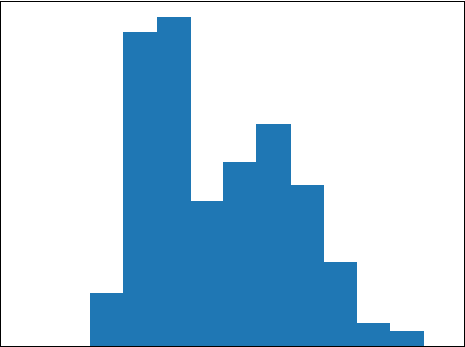
\includegraphics[width=.2\textwidth]{part2/figures/WAKE/discrete.pdf}};
    \node [inner sep=0pt] (cont) at (-2,3.1) {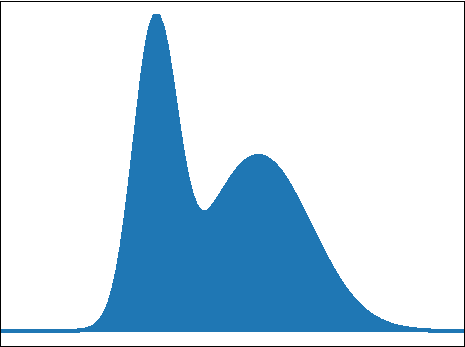
\includegraphics[width=.2\textwidth]{part2/figures/WAKE/continuous.pdf}};
    \draw[-stealth] (cont) to [bend left] (A);
    \draw[-stealth] (disc.east) to [bend right] (B);
    % Text
    \node at (5, 0.25) {$\mathcal{H}_k$};
    \node at (-3, 3) {$P$};
    \node at (-3, 1) {$Q$};
\end{tikzpicture}
    \caption{Kernel mean embedding of two probability distributions $P$ and $Q$ mapped in the $RKHS$  $H_k$}
    \label{fig:kernel_embedding}
\end{figure}

The distance between the two kernel mean embeddings $\mu_P$  and $\mu_Q$ is called the maximum mean discrepancy (MMD). 
This distance between two distributions $P$ and $Q$ is initially defined by the worst-case error for any function within a unit ball of a Hilbert space $\iH_k$, generated by the kernel $k$:

\begin{equation}
\mathrm{MMD}_k(P,Q):=\underset{\| g \|_{\iH_k} \leq 1}{\mathrm{sup}} 
\left\lvert \int_{\mathbb{R}^d}{g(\bx) \mathrm{d}P(\bx)}
- \int_{\mathbb{R}^d}{g(\bx) \mathrm{d}Q(\bx)} \right\rvert
= \|\mu_P(\bx) - \mu_Q(\bx) \| _ {\iH_k}.
\end{equation}
The MMD fully relies on the difference of kernel mean embeddings. 
Moreover, according to \cite{sriperumbudur_2010}, a kernel is called “characteristic kernel” when the following equivalence is true, $MMD_k (P,Q)=0 \iff P=Q$, making the MMD a metric on $\mathbb{R}^d$. 
For its good convergence behavior, the squared MMD has been used for multiple other purposes than numerical integration: statistical testing \cite{gretton_2006}, sensitivity analysis \cite{daveiga_2015}. 
When elevated to the square, it can be estimated using one $n$-sized representative sample of $P$ denoted $\left\{ \bx^{(i)} \right\}_{i \in (1,..,n)}$
(and respectively one $m$-sized sample of $Q$ denoted $\left\{ \by^{(i)} \right\} _{i \in (1,..,m)}$:

\begin{equation}
\widehat{\mathrm{MMD}_k}(P,Q) ^ 2 = \frac{1}{n^2} 
\sum_{i,j=1}^{n}{k(\bx^{(i)}, \bx^{(j)})} - \frac{2}{n m} \sum_{i=1}^{n}{ } \sum_{j=1}^{m}{k(\bx^{(i)},\by^{(j)})} + \frac{1}{m^2}  \sum_{i,j=1}^{m}{k(\by^{(i)},\by^{(j)})}.
\end{equation}
In the following, the idea is to compare the ambient wind distribution $p_0$ to the wake-perturbed wind conditions $p_l'$ at the WT~$l$ using the previously defined squared MMD.

%------------------------------------------------------------%
\paragraph{Application to the South Brittany wind farm project}
\label{SecApplicationSB}
%------------------------------------------------------------%
Once the joint perturbed distributions of each WT are estimated by a large Monte Carlo sample (cf. section~\ref{sec:UQ-wake}), the MMD with the ambient wind conditions can be computed. 
Figure~\ref{FIGWakeEffect} illustrates for each WT the squared MMD value computed to measure the wake-induced perturbation. 
Let us remind that MMD is a distance between the joint perturbed distribution at a WT computed for all wind orientations with the ambient wind distribution. 
Despite the wake obviously depend on the wind direction, our final goal is to define a small number of WT for RBD thus independently of the wind orientation. 
The lower this metric gets, the closer to the ambient wind distribution. 
Quite logically, the WT in the center of the farm are more affected by the wake since they are subject to the wake regardless of the wind direction.

The values of squared MMD given in the previous figure are estimated between two samples:
\begin{itemize}
    \item the Monte Carlo sample of the free environmental distribution: $\bX_n$,
    \item the wake-perturbed Monte Carlo sample at the WT $l: \bX'_{n,l}$ (output of the steady-state wake numerical model).
\end{itemize}

To ensure that the Monte-Carlo estimation converged, Figure~\ref{FIGConvergenceMMD} plots the squared MMD between the sample $\bX_n$ and the increasing samples $\bX'_{i,l},i \in {400,..,6000}$. 
After a few thousands of simulations, the MMD of each WT tends to converge towards a stable value, as expected. 
The design of experiment with $n=6~000$ is thus considered as sufficient. 

\begin{figure}
    \centering
    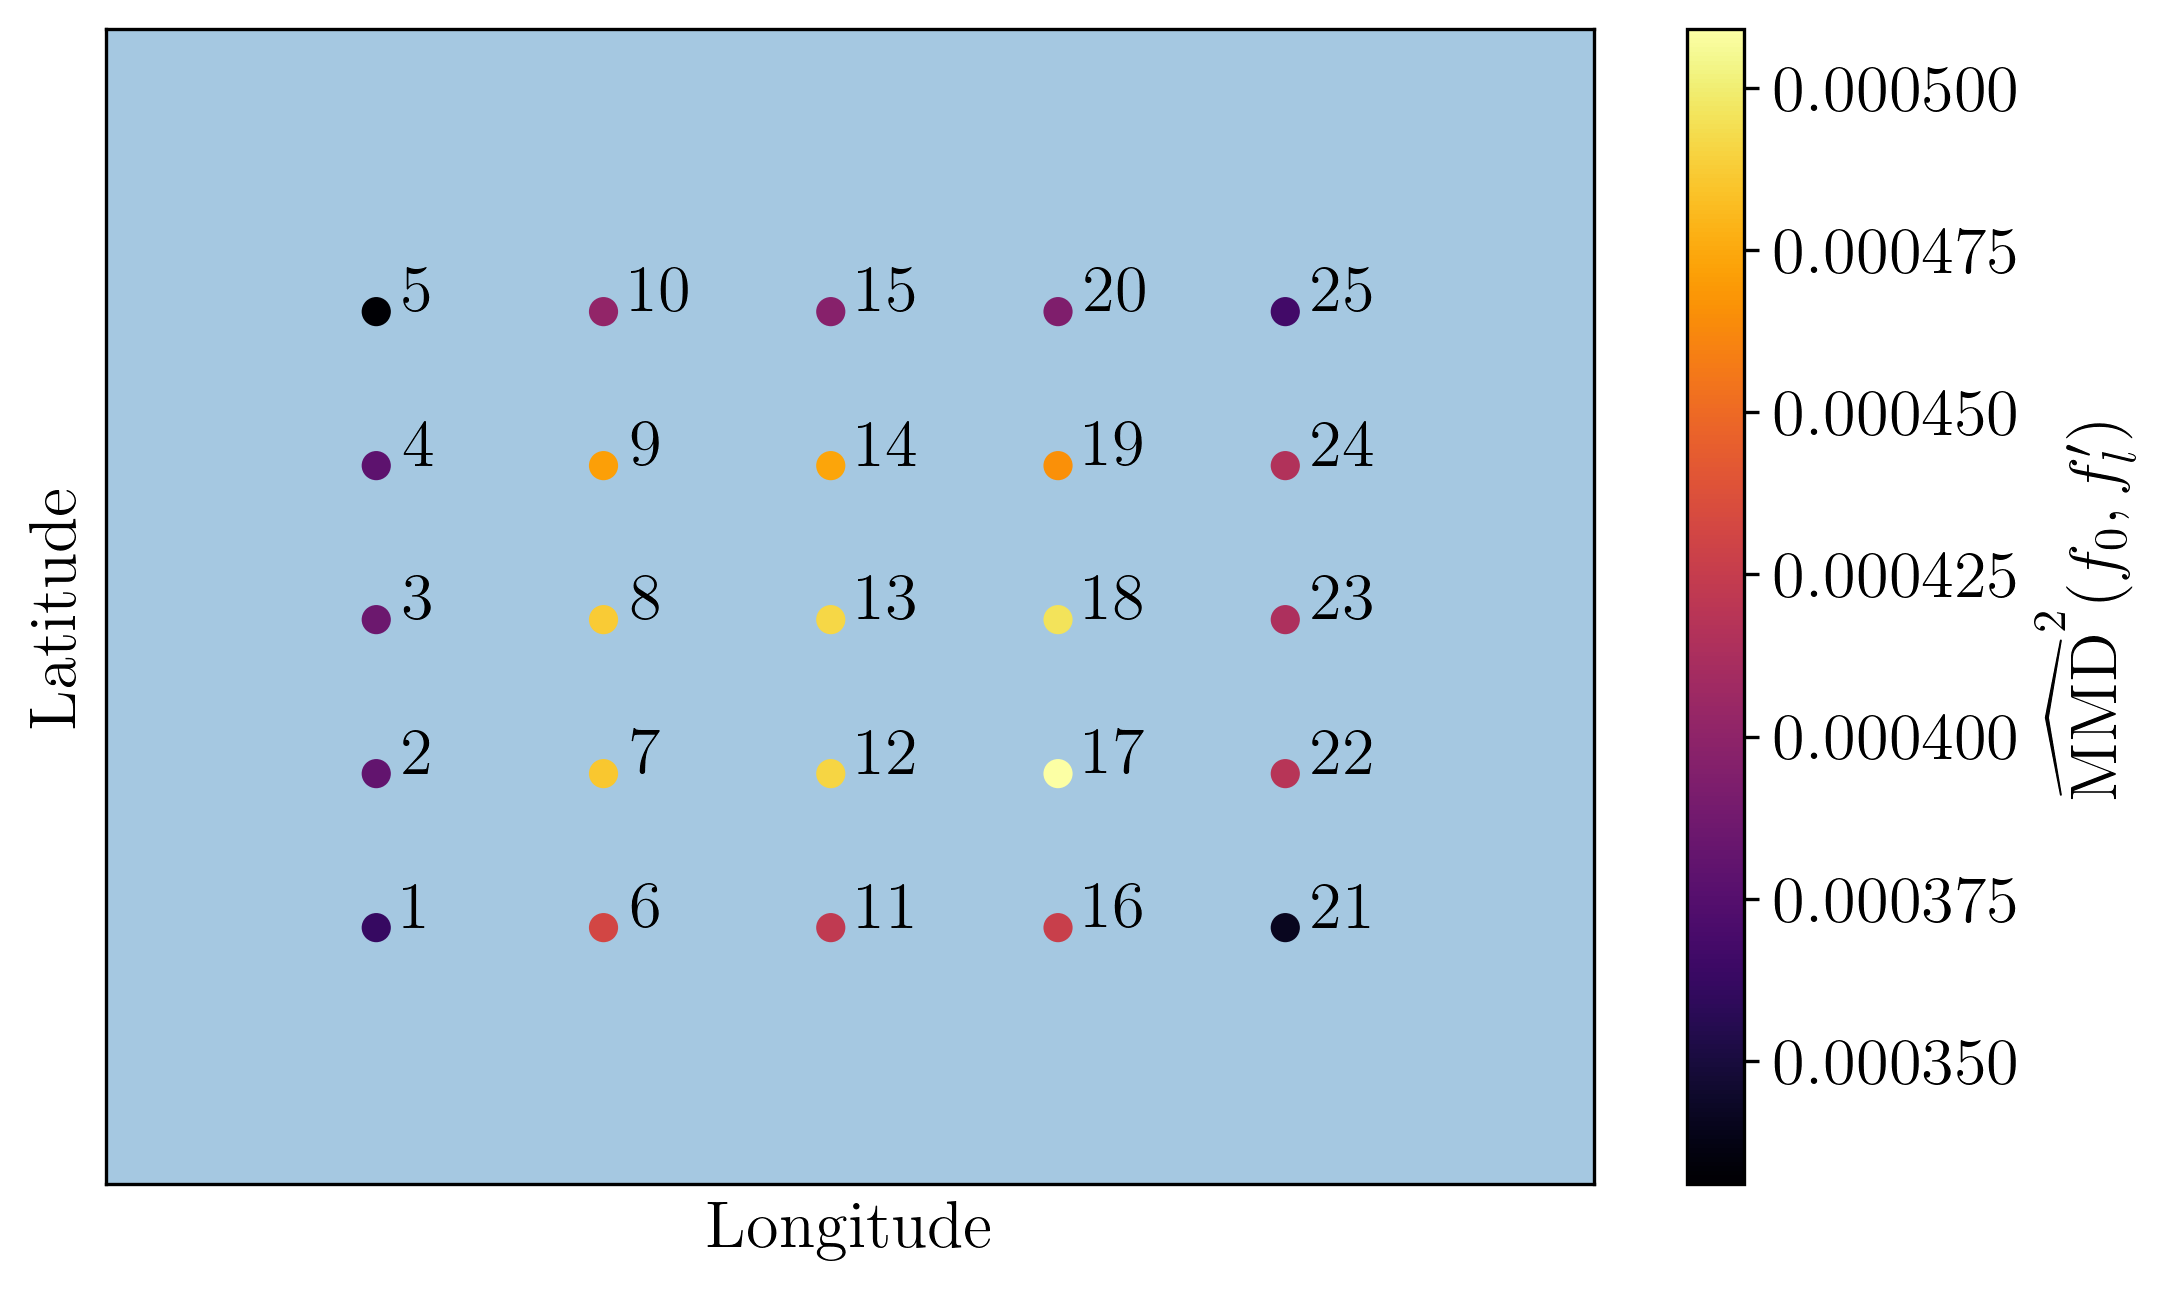
\includegraphics[width=0.6\textwidth]{part2/figures/WAKE/wake_perturbation_SB.png}
    \caption{South Brittany layout and wake effects measured by the squared MMD on wind conditions. 
    Note that the vertical direction on this plot does not represent the north direction.}
\label{FIGWakeEffect}
\end{figure}

\begin{figure}
    \centering
    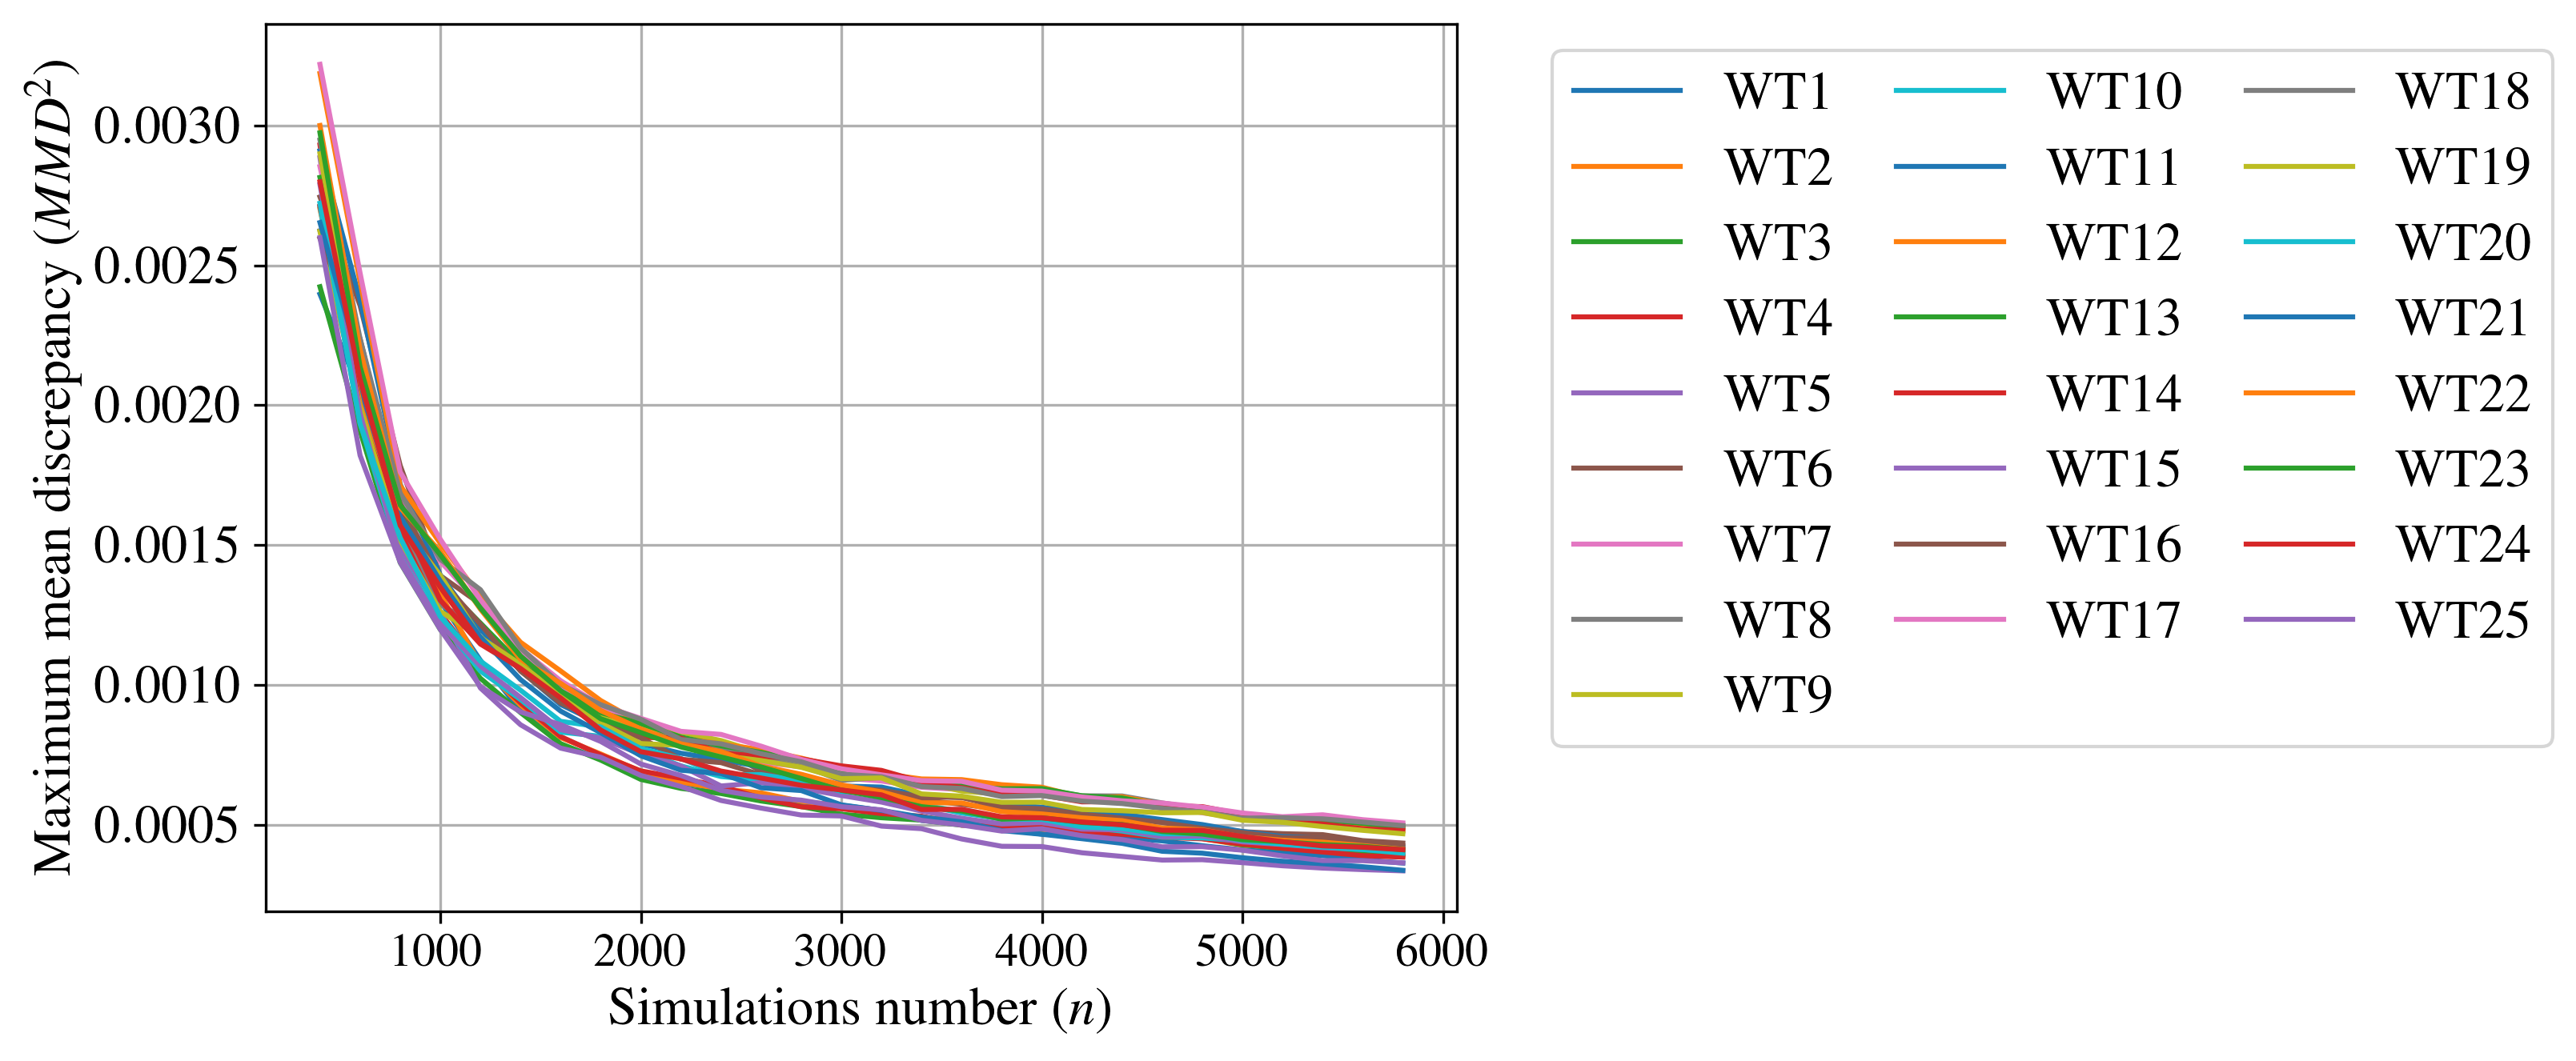
\includegraphics[width=0.7\textwidth]{part2/figures/WAKE/convergence_MC_SB.png}
    \caption{Convergence of the squared MMD estimation}
\label{FIGConvergenceMMD}
\end{figure}

%============================================================%
\subsection{Summary and discussion}
%============================================================%
A steady-state engineering wake model is coupled with a hydrostatic solver to take into account the effect of the floaters position in the wake computation of a floating offshore wind farm
The main impact of the floater's position is the increased rotor tilt, which leads to a larger vertical deflection of the wake. 
In the South-Brittany farm, the elevation of wake center is significant and could modify the fatigue loads on the downstream WT. 
This low-fidelity, or engineering model is very fast (about 3 minutes on a regular computer), while higher fidelity models can simulate the wake in a wind farm more accurately, but with much higher computational cost (several days for LES Meso-NH solver, with intensive parallelisation). 
In this paper, we consider that the modelling error made by the engineering wake model as reasonable. 
Further investigations should be done on the integration of the different fidelity levels in the uncertainty propagation. 
In this work, the uncertainty propagation is performed for to random inputs: the wind speed and the turbulence intensity, leading to a wake perturbed distribution per WT. 
A metric was then defined to measure the distance between distributions in order to build clusters of WT seeing similar wind conditions. 
After applying the metric to the South Brittany case, a clustering approach is used to determine a limited number of WTs representing the farm for RBD. 
Several clustering methods are compared and provide similar results for the current case study. In this case, a solution with 4 clusters is a good compromise between low relative error with clusters and low number of clusters. 
Getting a low number of clusters allows us to reduce the number of representative WT on which a RBD study can be done to assess the RBD over the whole farm. 
The differences among a cluster and between clusters have to be studied when looking directly to the output of interest for ultimate or fatigue reliability. 
However the difference on load output quantities may be reduced when compared to that on wake output quantities thanks to the damping of the WT. 
Depending on the definition of a wind farm failure (series system: one WT fails or parallel system: all WT fail or intermediate system), the probability of failure can be estimated from the probability of failure of the representative WT. 
These considerations need to be further explored to improve RBD at the farm scale. 


%============================================================%
%============================================================%
\section{Conclusion}
%============================================================%
%============================================================%